\chapter{Metodología}
%\chapter{Obtención de señales Bioeléctricas}
La metodología descrita a continuación contempla el proceso para la obtención de señales bioeléctricas con el equipo BIOPAC proporcionado en la UVG. 
Las señales bioeléctricas recopiladas en la UVG o brindadas por HUMANA, serán utilizadas para la implementación y evaluación de algoritmos de aprendizaje automático para el análisis y reconocimiento de segmentos de interés.

%\subsection{Filtro para BIOPAC MP41}
%Los equipos MP41 presentan un comportamiento extraño %al extraer los  datos, pasado 5 segundos sucede una caída de voltaje, luego esta se estabiliza sobre una horizontal por debajo de la original. Por lo que se le aplica un filtro pasa altas con frecuencia de corte de 10 Hz, de esta manera se recupera la señal sin afectar sus características como se observa en la Figura~\ref{fig:MP41_filtro}.

%\begin{figure}[t]
%    \centering
%    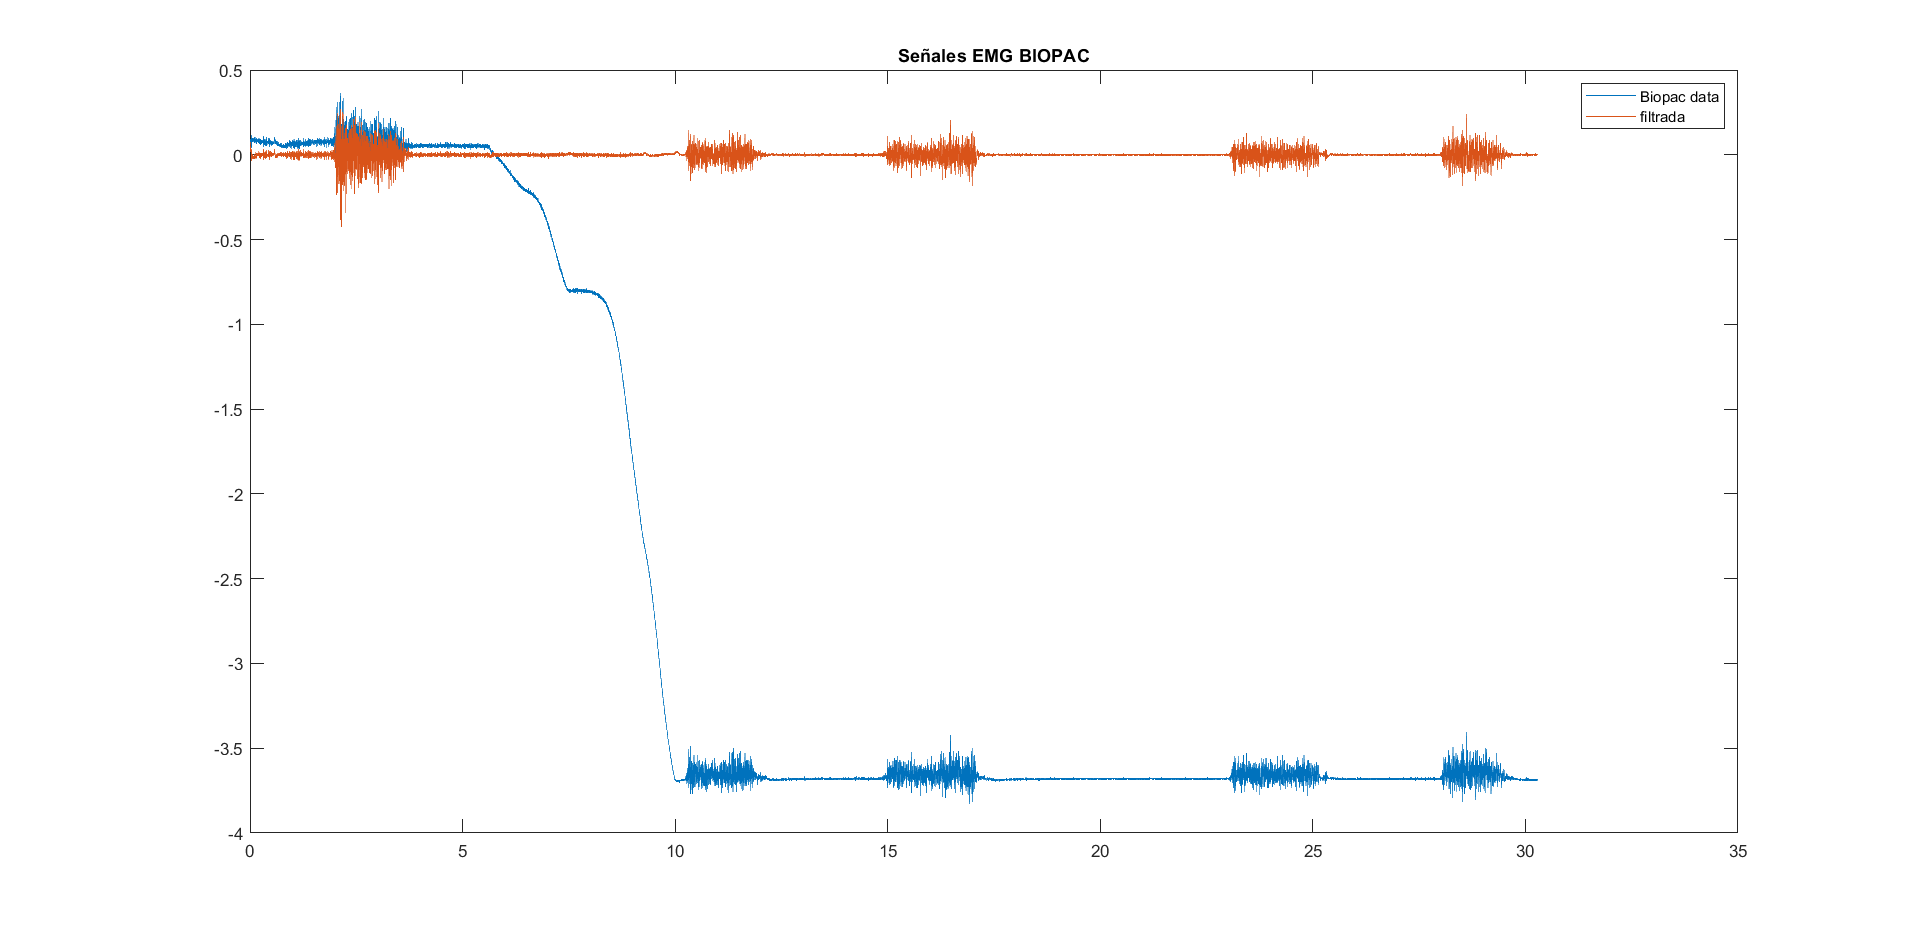
\includegraphics[width=0.9\textwidth]{figuras/10_filtro_MP41.png}
%    \caption{Señal original obtenido con MP41 (color azul) versus señal filtrada (color naranja).}
%    \label{fig:MP41_filtro}
%\end{figure}

\section{Datos obtenidos con equipo UVG}
En la Universidad del Valle de Guatemala se cuenta con los modelos MP36 y MP41 de BIOPAC, siendo el primero una versión más completa y de escritorio, mientras que el segundo es una versión portátil. Utilizando el equipo MP36 y MP41, se recopilaron señales del tipo EEG y EMG. Para cada tipo de señal bioeléctrica se tuvo un mínimo de tres sets diferentes de acciones por individuo.

\subsection{Señales EMG}
Para las señales EMG, el sujeto de prueba debía de encontrarse en estado de relajación. La pose del brazo en dicho estado se puede observar en la Figura~\ref{fig:relax_emg}.
Las grabaciones tuvieron una duración mínima de un minuto. Las personas mantuvieron la pose de relajación durante 2 segundos y posteriormente, durante otros 2 segundos realizaron la actividad solicitada, esto iteradas veces hasta cumplir con el mínimo de tiempo establecido. Las actividades fueron:

\begin{figure}[t]
    \centering
    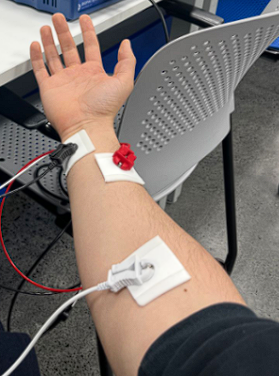
\includegraphics[width=0.2\textwidth]{figuras/16_emgRelax.png}
    \caption{Pose de relajación para toma de señales EMG con equipo BIOPAC.}
    \label{fig:relax_emg}
\end{figure}

\begin{figure}[t]
    \centering
    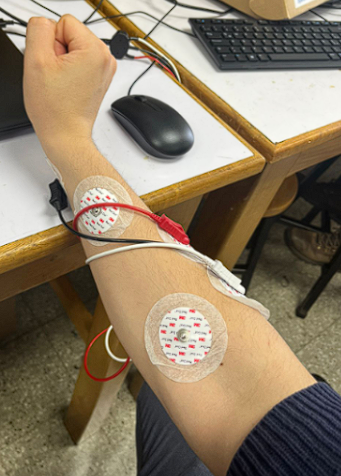
\includegraphics[width=0.2\textwidth]{figuras/17_elevarmunieca.png}
    \caption{Pose de actividad 1 en toma de grabación señal EMG.}
    \label{fig:actividad1_emg}
\end{figure}

\begin{figure}[H]
    \centering
    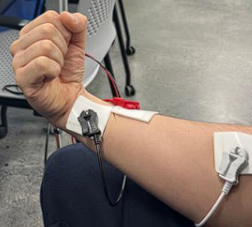
\includegraphics[width=0.2\textwidth]{figuras/19_contraer_munieca.png}
    \caption{Pose de actividad 2 en toma de grabación señal EMG.}
    \label{fig:actividad2_emg}
\end{figure}

\begin{figure}[H]
    \centering
    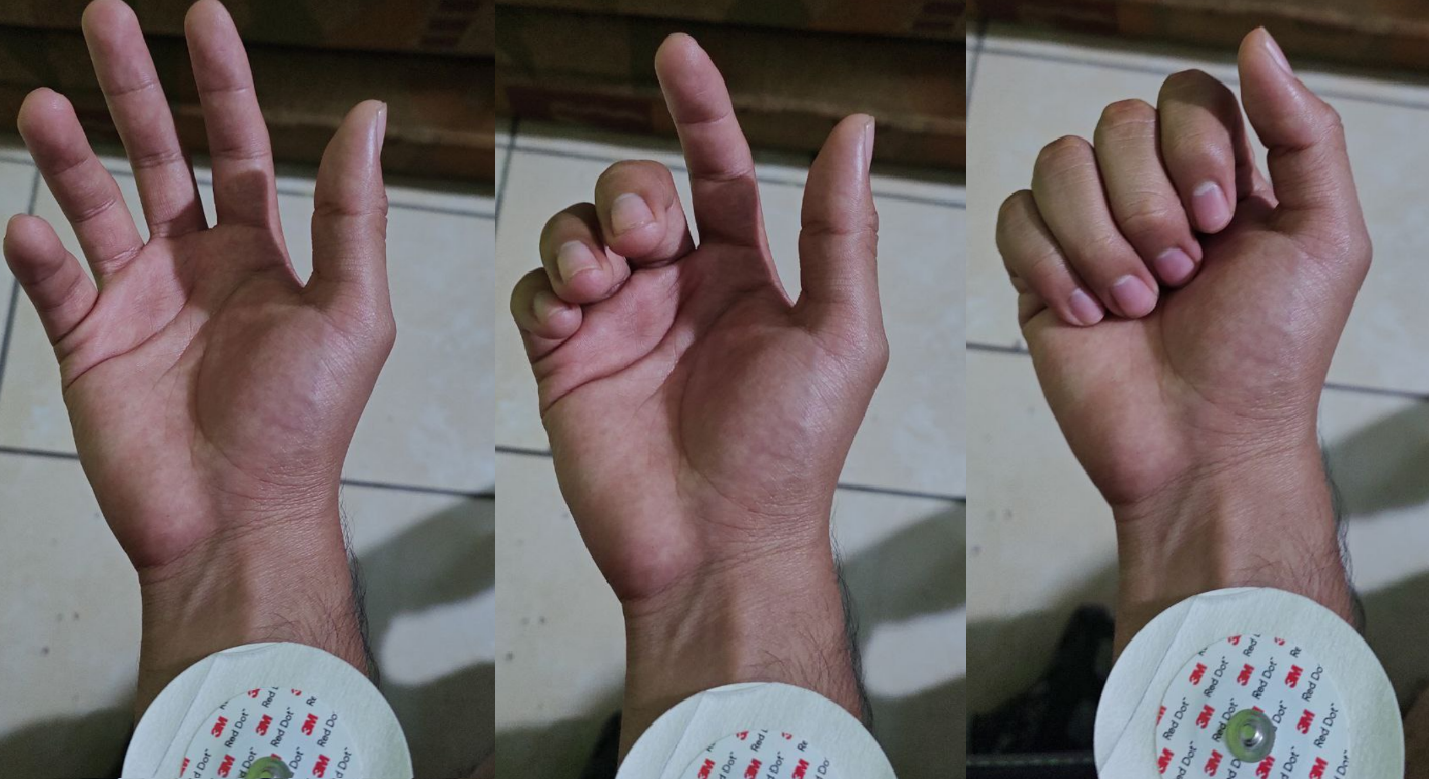
\includegraphics[width=0.3\textwidth]{figuras/18_empuniar.png}
    \caption{Pose de actividad 3 en toma de grabación señal EMG.}
    \label{fig:actividad3_emg}
\end{figure}

\begin{itemize}    
    \item Actividad 1:
    Elevar la muñeca hacia el exterior del cuerpo, como se observa en la Figura~\ref{fig:actividad1_emg}.    
    \item Actividad 2:
    Contraer la muñeca hacia el interior del cuerpo, como se observa en la Figura~\ref{fig:actividad2_emg}.     
    \item Actividad 3:
    Contraer paulatinamente cada uno de los dedos de la mano hacia el interior de la palma, como se observa en la Figura~\ref{fig:actividad3_emg}.    
\end{itemize}



\subsection{Señales EEG}
Para las señales EEG, el sujeto de prueba debía de encontrarse en estado de relajación, lo cual implicaba ojos cerrados y haber realizado al menos 3 repeticiones de inhalación y exhalación profundas.
Las grabaciones tuvieron una duración mínima de un minuto. Las personas mantuvieron la pose de relajación durante al menos 30 segundos al inicio, posteriormente se procedió a realizar una de las actividades especificas. Las actividades fueron:

\begin{itemize}    
    \item Actividad 1:
    Abrir los ojos durante 10 segundos y luego, volver a cerrar los ojos durante otros 10 segundo.       
    \item Actividad 2:
    Abrir los ojos y realizar una prueba matemática nivel medio, la cual consistía en sumas, restas, multiplicaciones y divisiones de números enteros de hasta 7 dígitos.    
    \item Actividad 3:
    En los trabajos de graduación presentados por Margareth Vela \cite{magy_2023} y Oscar Fuentes \cite{oscar_2023}, los cuales consistieron en el estudio cualitativo y cuantitativo del impacto de los pulsos binaurales en el estado de ánimo, concentración y calidad del sueño de las personas y aplicación de técnicas de aprendizaje automático y reconocimiento de patrones en las señales bioeléctricas. Se realizaron las actividades 1 y 2 nuevamente pero ahora, mediante audífonos se aplicaron pulsos binaurales.    
    \item  Actividad 4:
    Esta expresión involucra activar los músculos ubicados en la frente con el fin de levantar las cejas de forma rítmica y deliberada, tal como se evidencia en la Figura~\ref{fig: eeg_actividad4}.    
    \item Actividad 5:
    Inclinación de la cabeza hacia abajo. Este movimiento implica girar la cabeza hacia abajo, en dirección al pecho o hacia el suelo, como se ilustra en la Figura~\ref{fig: eeg_actividad5}.    
    \item Actividad 6:
    Inclinación de la cabeza hacia arriba. Este movimiento implica girar la cabeza hacia arriba, en dirección contraria al pecho, como se ilustra en la Figura~\ref{fig: eeg_actividad6}.    
    \item Actividad 7:
    Inclinación de la cabeza. Este movimiento consiste en girar la cabeza hacia la derecha, como se ilustra en la Figura~\ref{fig: eeg_actividad7}.
\end{itemize}

\begin{figure}[H]
	\centering
	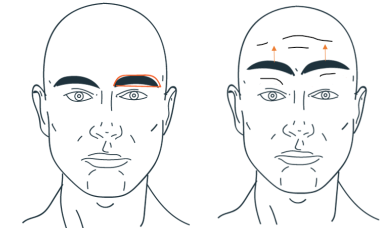
\includegraphics[width=0.3\textwidth]{figuras/40_cejas_arriba.png}
	\caption{Actividad 4 movimiento controlado de cejas.}
	\label{fig: eeg_actividad4}
\end{figure}

\begin{figure}[H]
	\centering
	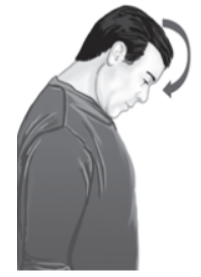
\includegraphics[width=0.15\textwidth]{figuras/41_head_down.png}
	\caption{Actividad 5 inclinación de la cabeza hacia abajo.}
	\label{fig: eeg_actividad5}
\end{figure}

\begin{figure}[H]
	\centering
	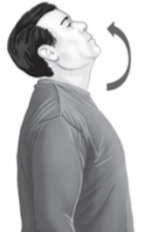
\includegraphics[width=0.15\textwidth]{figuras/42_head_up.png}
	\caption{Actividad 6 inclinación de la cabeza hacia arriba.}
	\label{fig: eeg_actividad6}
\end{figure}

\begin{figure}[H]
	\centering
	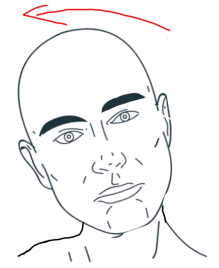
\includegraphics[width=0.2\textwidth]{figuras/43_inclinar.png}
	\caption{Actividad 7 inclinación de la cabeza hacia el lateral derecho.}
	\label{fig: eeg_actividad7}
\end{figure}

\subsection{Estándar en recolección de datos BIOPAC}
Se definió un documento estándar de formato ``.xlsx'' para el almacenamiento de las señales EMG y EEG obtenidas con el equipo BIOPAC,  como se observa en la Figura~\ref{fig:Estandar_bipoac_uvg}. Los datos principales que se necesitan son:

\begin{figure}[H]
    \centering
    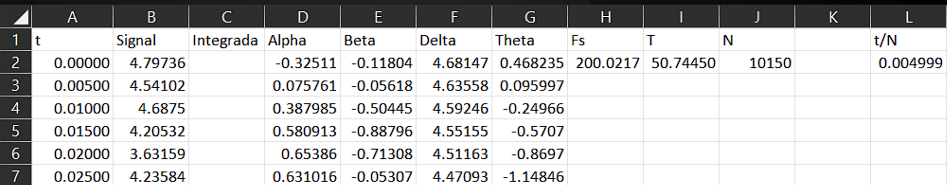
\includegraphics[width=0.9\textwidth]{figuras/11_estandar_biopac_uvg.png}
    \caption{Estándar para el almacenamiento de datos obtenidos con el equipo BIOPAC de la UVG.}
    \label{fig:Estandar_bipoac_uvg}
\end{figure}

\begin{itemize}
    \item Señal (signal)
    \item Tiempo de grabación (T)  
    \item Número de muestras (N)
\end{itemize}

La primer columna llamada ``t'' se auto genera al llenar los datos principales y consiste en el tiempo en el que se obtuvo la señal que se encuentra en la columna ``\textit{Signal}''. 
El parámetro que se encuentra en la columna ``Fs'' corresponde a la frecuencia de muestreo la cual se auto calcula.
El parámetro que se encuentra en la columna ``t/N'' corresponde al tiempo dividido numero de muestras la cual se auto calcula, esto permite marcar la diferencia de tiempo que hay entre una muestra y la siguiente.

Las columnas siguientes son opcionales ya que dentro de la herramienta de software para el estudio de la epilepsia no se hace uso de ellas. Por lo que siempre habrá al menos una de estas columnas en blanco, ya que se llenan acorde al tipo de señal bioeléctrica a recolectar. Estas columnas son:
\begin{itemize}
    \item Integrada: es el área situada bajo la curva de la señal EMG rectificada, lo que equivale a la integral matemática del valor absoluto de la señal EMG original \cite{BIOPAC}.
    \item Alpha: señal EEG filtrada para observar frecuencias de 8 Hz a 12 Hz.
    \item Beta: señal EEG filtrada para observar frecuencias de 12 Hz a 30 Hz.
    \item Delta: señal EEG filtrada para observar frecuencias de 1 Hz a 4 Hz.
    \item Theta: señal EEG filtrada para observar frecuencias de 4Hz a 8 Hz.
\end{itemize}


Tras recolectar estos datos la norma de almacenamiento consiste en, nombrar el documento con el nombre y apellido de la persona a la que se le extrajo las señales bioeléctricas, seguido de un guion (bajo o normal), el tipo de actividad que se realizó y por último, el tipo de señal bioeléctrica que se extrajo. En la Figura~\ref{fig:dataCruda_almacenada} se observa un ejemplo de ello.

\begin{figure}[H]
    \centering
    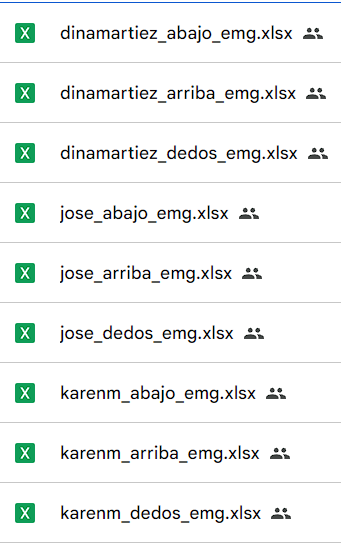
\includegraphics[width=0.30\textwidth]{figuras/20_datosCrudo_norma.png}
    \caption{Señales bioeléctricas extraídas con el equipo BIOPAC almacenadas según la norma establecida.}
    \label{fig:dataCruda_almacenada}
\end{figure}

\subsection{Estructuración de los datos para ser usados en la herramienta de software para el estudio de la epilepsia}
Para los datos obtenidos con el equipo BIOPAC de la UVG, es necesario convertirlos en un formato tipo \textit{\gls{Struct}}, de esta manera se podrá usar dicha información dentro de la la herramienta de software para su análisis y estudio, como se muestra en la Figura~\ref{fig:struc_func}. 

\begin{figure}[H]
    \centering
    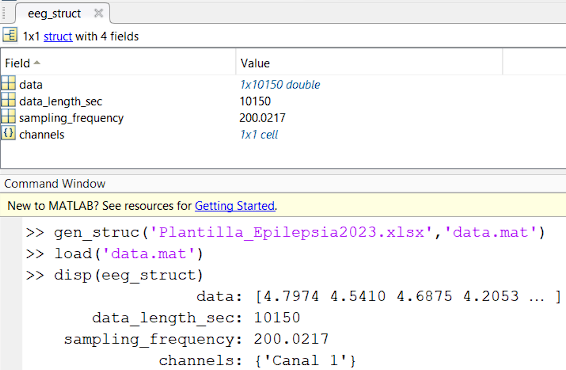
\includegraphics[width=0.6\textwidth]{figuras/12_struct_funct.png}
    \caption{Contenido de \textit{struct} para el uso de datos dentro de la herramienta de software para el estudio de la epilepsia.}
    \label{fig:struc_func}
\end{figure}

Para ello se creo la función ``gen\_struc'' la cual, posee como primer argumento el nombre del documento a extraer los datos y como segundo argumento el nombre y el formato con el que se almacenará el \textit{struct}. Dicho formato contiene los siguientes espacios:
\begin{itemize}
    \item Datos (mV)
    \item Cantidad de datos
    \item \gls{Frecuencia de muestreo} (Hz)
    \item Cantidad de canales
\end{itemize}

\section{Datos de HUMANA de pacientes con epilepsia }
HUMANA ha compartido 4 grabaciones de señales EEG, la información de dichas grabaciones se puede ver en el Cuadro~\ref{cuadro:tabla_edf_info}. Estos datos fueron de ayuda para el entrenamiento y verificación de exactitud de los modelos de aprendizaje automático. 

\begin{table}[H]
\begin{center}    
    \begin{tabular}{|l|l|l|l|l|}
    \hline
    \multicolumn{1}{|c|}{\textbf{Nombre}} & \multicolumn{1}{c|}{\textbf{Canales}} & \multicolumn{1}{c|}{\textbf{Duración}} & \multicolumn{1}{c|}{\textbf{Frecuencia de muestreo}}\\ %\hline
          &  & (hh:mm:ss) & \\ \hline
    AL.edf  & 33  & 03:01:56 & 200 Hz   \\ \hline
    CLEA.edf& 29  & 02:39:42 & 200 Hz   \\ \hline
    GIKA.edf& 29  & 02:58:06 & 200 Hz   \\ \hline
    HCHC.edf& 29  & 23:02:44 & 200 Hz   \\ \hline
    Ajczalar M.edf& 30  & 15:57:13 & 300 Hz   \\ \hline
    GUADRON T.edf& 30  & 03:02:01 & 300 Hz   \\ \hline
    \end{tabular}
    \caption[Información de grabaciones dadas por HUMANA]{Información de grabaciones de señales bioeléctricas de pacientes con epilepsia brindadas por HUMANA.} 
    \label{cuadro:tabla_edf_info}
\end{center}
\end{table}

\section{Agrupamiento de datos}
Con el equipo UVG se recopilaron señales bioeléctricas del tipo EEG y EMG, las cuales se agruparon de forma \gls{intersujeto} e \gls{intrasujeto} respectivamente. En el caso de señales brindadas por HUMANA estas no necesitan agrupación, ya que por lo general son de una duración mayor a una hora de grabación contando como mínimo 29 canales, por lo que esto ya son datos suficientes para proceder a realizar su análisis.

El análisis de señales EEG de forma intersujeto y señales EMG de forma intrasujeto se realiza de esta manera debido a las diferencias fundamentales en la naturaleza de estas dos tipos de señales y los objetivos específicos de análisis en cada caso.

\subsection{Análisis de señales EEG de forma intersujeto}
Las señales EEG, que representan la actividad eléctrica del cerebro, tienden a mostrar una variabilidad significativa entre diferentes individuos. Las diferencias en la anatomía cerebral, la disposición de electrodos, la edad y otros factores pueden influir en las características de las señales EEG. Por lo tanto, se suele analizar de forma intersujeto para comprender cómo varían las respuestas entre diferentes personas.

El análisis intersujeto de las señales EEG es relevante en aplicaciones clínicas y de investigación que involucran poblaciones de pacientes o participantes diversos. Permite identificar patrones generales en grupos de personas y puede ayudar en la detección de trastornos neurológicos como la epilepsia en una población más amplia.

\subsection{Análisis de señales EMG de forma intrasujeto}
Las señales EMG, que registran la actividad eléctrica de los músculos, tienden a mostrar menos variabilidad intrasujeto, es decir, las características de la señal son relativamente consistentes en un individuo específico a lo largo del tiempo. Esto se debe a que la anatomía y la disposición de los músculos de una persona tienden a ser estables.


\section{Aprendizaje automático}
En la presente sección se presentan los algoritmos y métodos que se usaron para medir la efectividad de los algoritmos en el reconocimiento de patrones en señales bioeléctricas que sean de interés. 

\subsection{Extracción de características}
Se extrajeron características en el dominio del tiempo, la frecuencia y \gls{wavelets} de cada uno de los conjuntos de datos obtenidos mediante el equipo UVG o proporcionados por HUMANA. Se aplicó la transformada a cada dominio a las señales, seguida de la extracción de características. A partir de este punto, estas características obtenidas mediante las transformadas serán referidas simplemente como ``características frecuencia'', ``características tiempo'' o ``características wavelets'' por conveniencia. Este proceso de extracción de características fue analizado detalladamente con el objetivo de optimizar el tiempo de entrenamiento de los algoritmos de aprendizaje automático y, en la medida de lo posible, mejorar la clasificación de las señales bioeléctricas.

\subsection{Anotaciones automáticas}
Empleando los algoritmos de aprendizaje automático desarrollados en las fases anteriores, se clasificó la señal bioeléctrica entre, ``Ictal'', ``Sano'', ``Interictal'' o Preictal'', según fuera su caso. A su vez, se implemento una sección para exportar los segmentos de interés a un documento CSV, como se puede observar en la Figura~\ref{fig:yo_anotaciones}.

\begin{figure}[H]
    \centering
    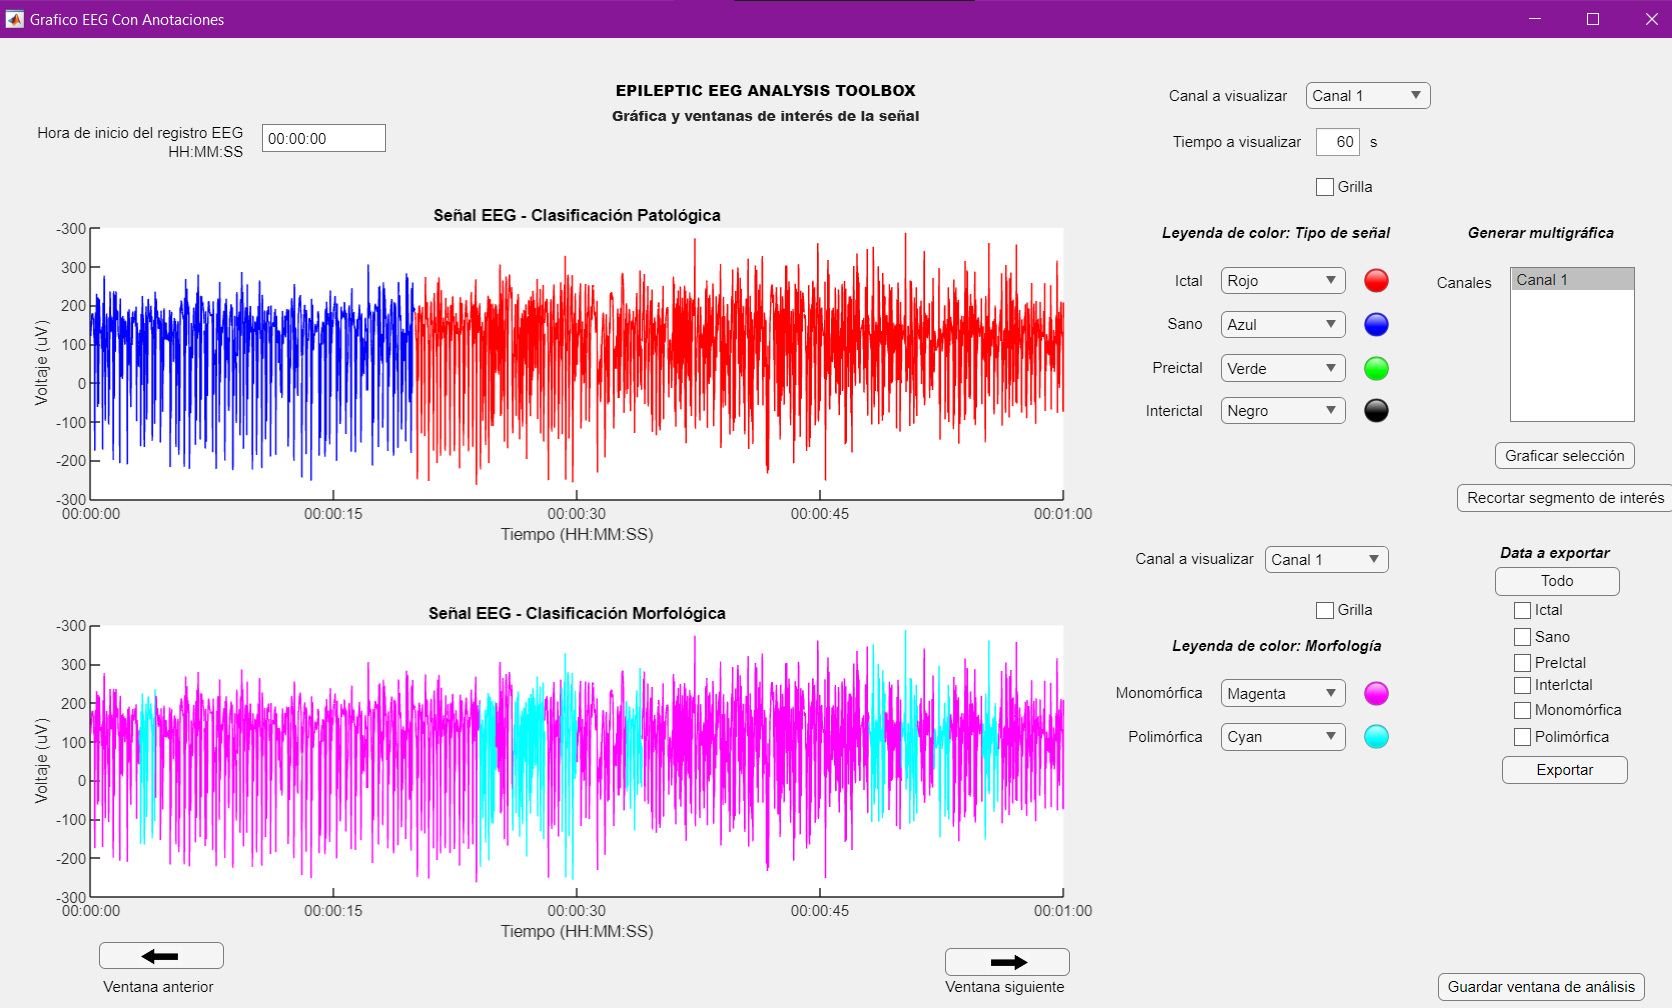
\includegraphics[width=0.6\textwidth]{figuras/13_modificacion_anotaciones.png}
    \caption{Ventana de anotaciones automáticas con nueva sección para exportar datos de interés.}
    \label{fig:yo_anotaciones}
\end{figure}

\subsection{Análisis estadístico}
Mediante matrices de confusión se validó la efectividad de las redes neuronales y las SVM (algoritmos de aprendizaje supervisado). Para el caso de los algoritmos de agrupamiento de \textit{K-means} y Jerárquico (algoritmos de aprendizaje no supervisado) se procedió a validar su efectividad mediante el algoritmo ``\textit{rand index}'', el cual es una medida de validez para algoritmos de agrupamiento. Además se tabularon tiempos relevantes, desde la extracción de características hasta la generación de anotaciones automáticas. 

\section{Actualización de la herramienta de software para el estudio de la epilepsia}
El primer paso para la actualización de la herramienta de software para el estudio de la epilepsia fue eliminar los mensajes de advertencia y arreglar errores que se encontraban dentro de la herramienta de software para el estudio de la epilepsia. En las Figuras~\ref{fig:yo_error_uno} y ~\ref{fig:yo_warning_uno} se puede observar algunos ejemplos, la mayoría de estos eran a causa de prácticas de programación no tan eficientes en MATLAB. 

\begin{figure}[t]
    \centering
    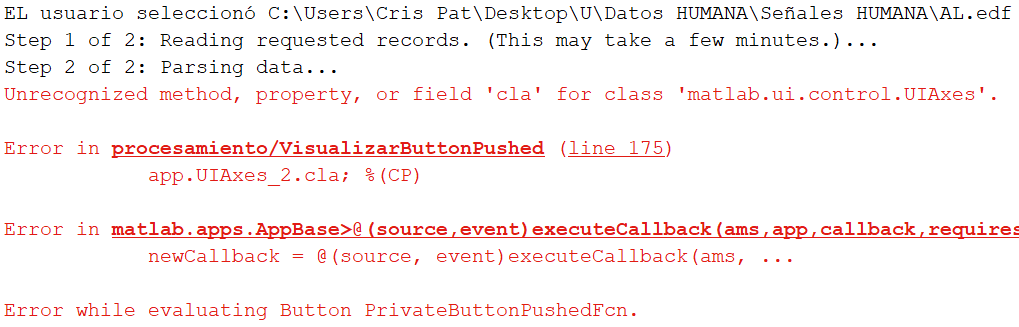
\includegraphics[width=0.65\textwidth]{figuras/14_AnalizaPrueba_visualizar.png}
    \caption{Error al utilizar botón de visualización de canales en la ventana de anotaciones automáticas.}
    \label{fig:yo_error_uno}
\end{figure}

\begin{figure}[t]
    \centering
    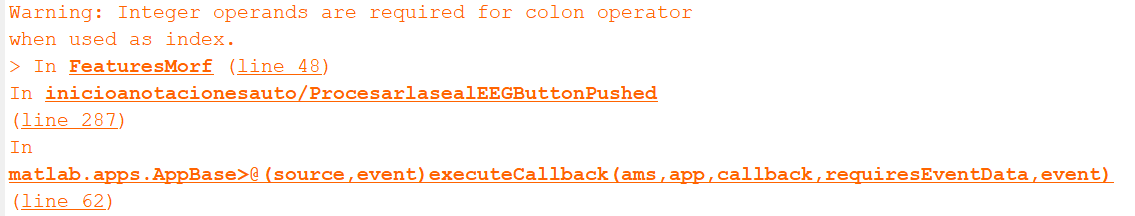
\includegraphics[width=0.65\textwidth]{figuras/15_alerta_feature_Morf.png}
    \caption{Alerta al emplear el algoritmo FeaturesMorf.}
    \label{fig:yo_warning_uno}
\end{figure}

En todos los casos al momento de extraer las características de las señales bioeléctricas, se tenía que no se pre-creaba el vector donde se almacenarían dichas características, además de contar con variables y condicionales innecesarias, como se puede observar en la Figura~\ref{flu:vfeatures malo}. Esto resulta ser computacionalmente costoso, lo que da paso a pérdida de tiempo innecesaria. Por lo que se procedió a corregirlo, creando el vector de características con las dimensiones máximas que podría tener, siendo la cantidad de filas del tamaño del vector de datos y la cantidad de columnas, del tamaño de las posibles características de interés, como se puede observar en la Figura~\ref{flu:vfeatures bueno}.

\begin{figure}[H]
    \centering
    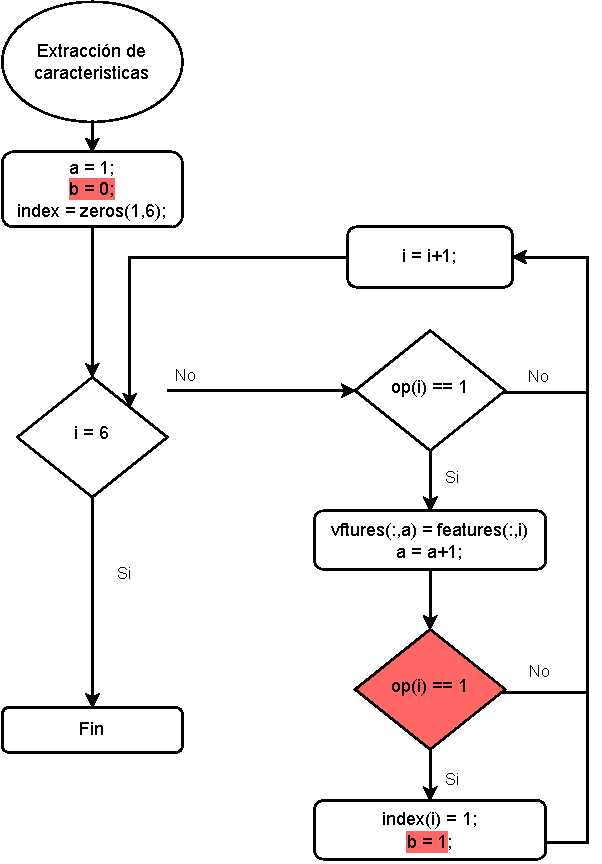
\includegraphics[width=0.5\textwidth]{figuras/21_flujograma_vfeatures_mal.pdf}
    \caption{Flujograma de la creación del vector de características versión 2022.}
    \label{flu:vfeatures malo}
\end{figure}

\begin{figure}[H]
    \centering
    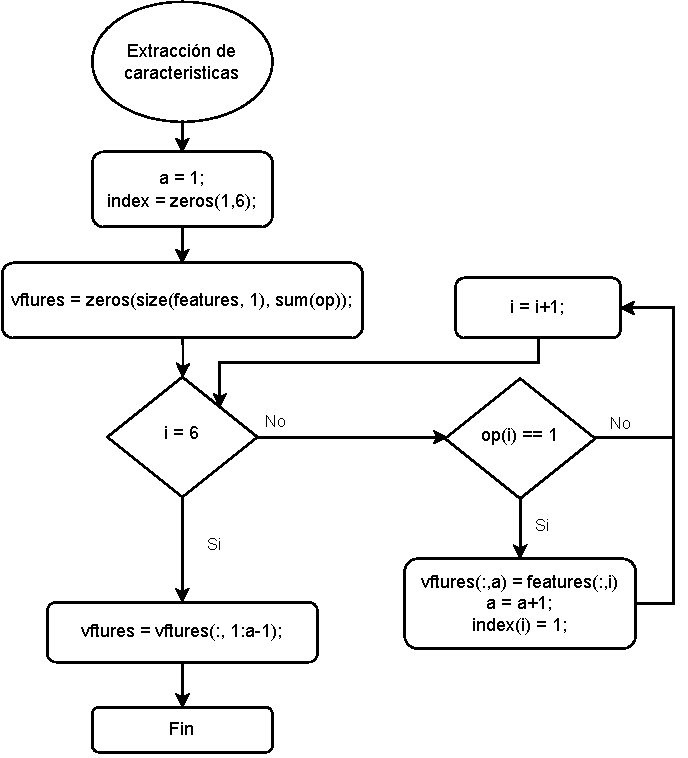
\includegraphics[width=0.5\textwidth]{figuras/22_flujograma_vfeatures_bien.pdf}
    \caption{Flujograma de la creación del vector de características versión 2023.}
    \label{flu:vfeatures bueno}
\end{figure}

Al momento de establecer rangos de datos a analizar por ventanas, se encontraba como limite superior la expresión de la Ecuación(\ref{eq: Limite superior vfeatures}), lo cual al tratarse de un vector los valores ingresados para los índices deben ser enteros, característica que no cumple el limite superior cuando la variable ``muestras'' es un número impar. Por lo que se procedió a redondear el valor al mínimo más próximo, dando la expresión de la Ecuación(\ref{eq: vfeatures_rango}). Un claro ejemplo de este proceso se puede observar en la Figura~\ref{fig: redondeo minimo}. 

\begin{equation}
    Lim\_sup = \frac{muestras}{2} + 1
    \label{eq: Limite superior vfeatures}
\end{equation}

\begin{equation}
    VectorVentana=VectorAnalizar(1:floor( \frac{muestras}{2} + 1));
    \label{eq: vfeatures_rango}
\end{equation}

\begin{figure}[H]
    \centering
    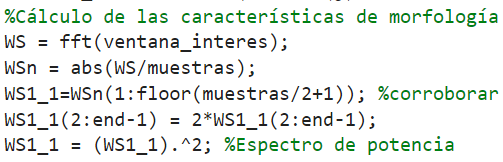
\includegraphics[width=0.45\textwidth]{figuras/23_redondeo_indicevector.png}
    \caption{Segmento de código para el calculo de características de una señal bioeléctrica.}
    \label{fig: redondeo minimo}
\end{figure}

En el proceso de generación de característica, el algoritmo para determinar el ``Zero Crossing'' (ZC) no era el más adecuado, dicho algoritmo se puede ver en la Figura~\ref{flu: ZC malo}. 
El algoritmo creaba variables que no se utilizaban, sin embargo, si se realizaban operaciones matemáticas con ellos, lo que implica tiempo y calculo computacional innecesario. A su vez, el algoritmo verificaba el cambio de signo directamente, sin usar el argumento ``umbral'', el cual es de gran relevancia ya que es este, quien permite el conteo adecuado de cambio de signo, sin tomar en cuenta aquellos cruces por cero que ocurren debido al ruido dentro de la señal. 
Por lo que se procedió a realizar las respectivas correcciones, como se muestra en la Figura~\ref{flu: ZC bueno}. En la presente versión se toma en cuenta el umbral para un correcto conteo, además de, ser una versión simplificada lo que lo hace más simple de realizar los cálculos computacionales.

\begin{figure}[H]
    \centering
    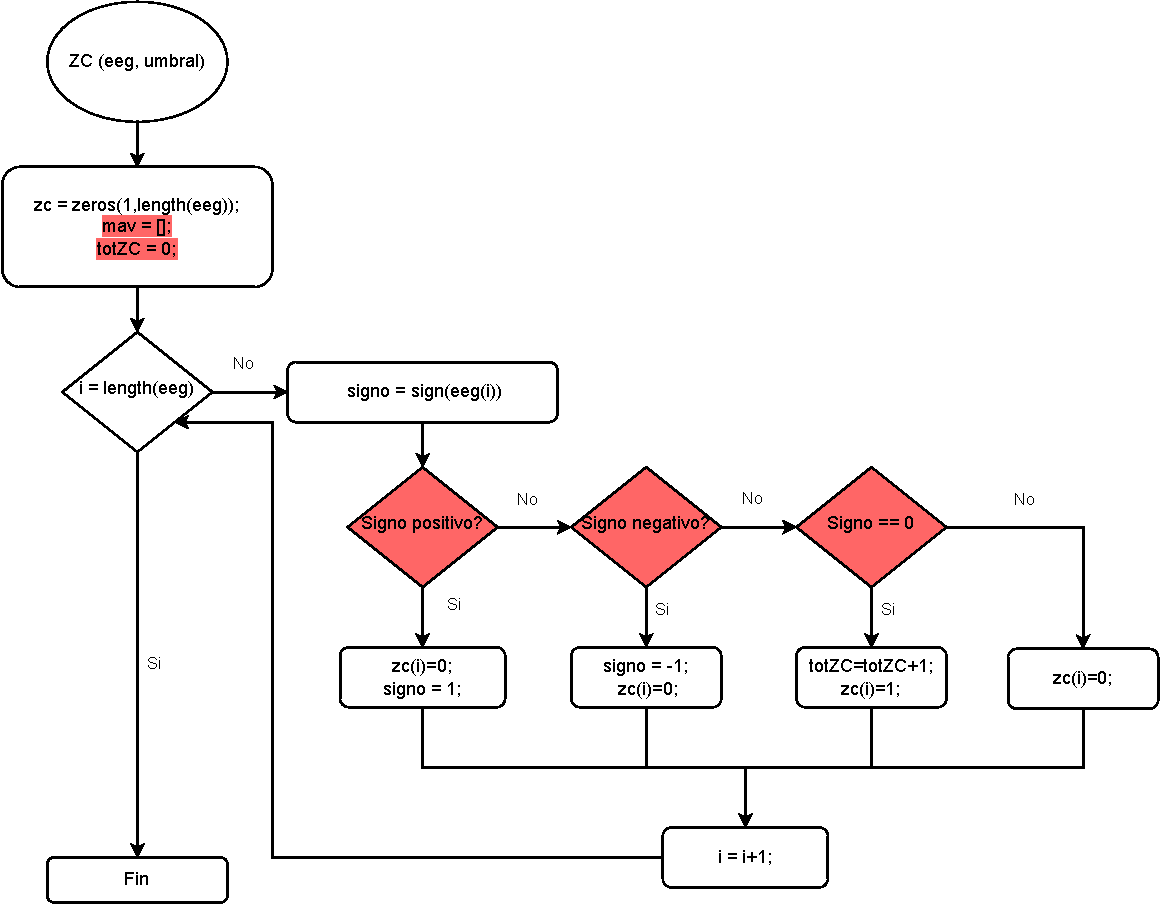
\includegraphics[width=0.75\textwidth]{figuras/24_flujograma_zc_mal.pdf}
    \caption{Flujograma de algoritmo ZC versión 2022.}
    \label{flu: ZC malo}
\end{figure}
\begin{figure}[H]
    \centering
    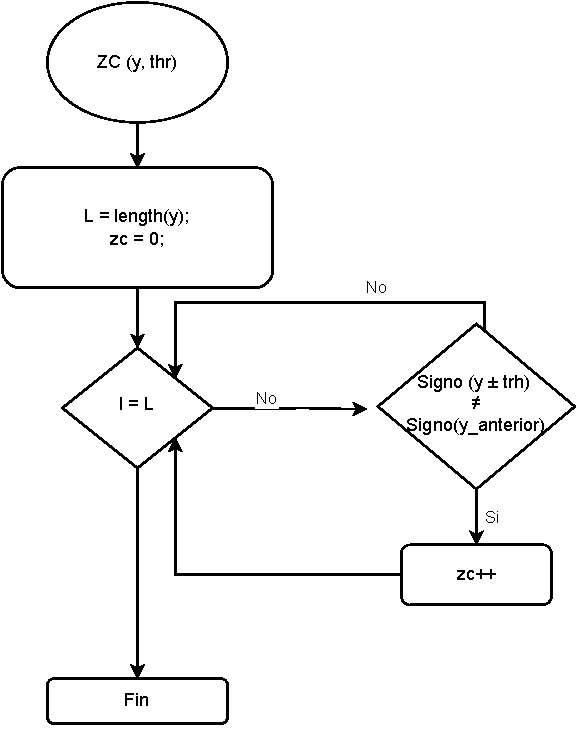
\includegraphics[width=0.5\textwidth]{figuras/25_flujograma_zc_bien.pdf}
    \caption{Flujograma de algoritmo ZC versión 2023.}
    \label{flu: ZC bueno}
\end{figure}

%-------------------------------------------------------
% A partir de aqui se discuten los resultados
%-------------------------------------------------------
\chapter{Resultados de recolección de datos}
En el presente capitulo se presentarán los datos de señales bioeléctricas obtenidas con el equipo de UVG y brindadas de HUMANA. Estas señales fueron la materia prima para la comprobación de funcionalidad de los algoritmos. En el capitulo de anexos, se incluyen los vínculos correspondientes a los datos recopilados.

\section{Señales Bioeléctricas obtenidas con el equipo de UVG}
La recolección de señales bioeléctricas con el equipo de UVG ha dado como resultado un total de 187 grabaciones, como se puede ver en el Cuadro~\ref{cuadro:tabla datos UVG}. Para el caso de las señales EEG, se cuenta con una duración promedio de 20 minutos por grabación. En el caso de las señales EMG, se cuenta con una duración promedio de 1 minuto por grabación. Por lo que ahora se cuenta con una base de datos de Señales EEG y EMG, recolectadas y procesadas en la Universidad del Valle de Guatemala.

En el Cuadro \ref{cuadro:tabla datos UVG} de datos recolectados, la categoría ``sin plantilla'' se refiere a grabaciones de señales bioeléctricas que no se guardaron con el ``Estándar en recolección de datos BIOPAC'', mientras que la categoría ``con plantilla'' hace referencia a grabaciones de señales bioeléctricas que sí utilizaban dicho estándar. 

\begin{table}[H]
\begin{center}
    \begin{tabular}{|l|l|l|l|l|}
    \hline
        \multicolumn{1}{|c|}{\textbf{Tipo}} & \multicolumn{1}{c|}{\textbf{Cantidad}} & \multicolumn{1}{c|}{\textbf{Formato}}\\ \hline
        EEG sin plantilla & 34  & XLSX \\ \hline
        EEG con plantilla & 18  & XLSX  \\ \hline
        EMG sin plantilla & 18  & XLSX y CSV \\ \hline
        EMG con plantilla & 117  & XLSX \\ \hline
    \end{tabular}
    \caption[Datos en nube con equipo UVG]{Datos recolectados con equipo UVG.} 
    \label{cuadro:tabla datos UVG}
\end{center}
\end{table}

Una vez organizado los datos obtenidos con el equipo de UVG, se procedió a generar los \textit{structs}, ya que este formato es el utilizado en la herramienta de software para el estudio de la epilepsia, siguiendo la norma que se describió en el capitulo anterior se almacenaron, se puede observar en la Figura~\ref{fig: Struct_normado}. Este formato permite extraer características de las grabaciones realizadas.

\begin{figure}[t]
    \centering
    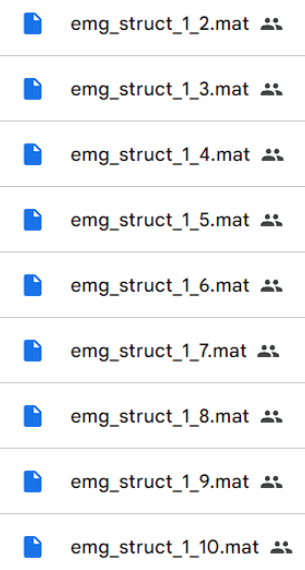
\includegraphics[width=0.15\textwidth]{figuras/29_strucs_normados.png}
    \caption{Structs generados a partir de los datos obtenidos con el equipo UVG.}
    \label{fig: Struct_normado}
\end{figure}

\subsection{Resultados de la Extracción de Características}
Para los datos recolectados se procedió a extraer sus características. Cabe mencionar que los datos que se obtuvieron con el equipo UVG son de personas que no padecen de epilepsia, teniendo un total de 10 vectores de características y 24 \textit{structs}, como se observa en el Cuadro~\ref{cuadro:tabla datos features UVG}.

\begin{table}[H]
\begin{center}
    \begin{tabular}{|l|l|l|l|l|}
    \hline
        \multicolumn{1}{|c|}{\textbf{Tipo}} & \multicolumn{1}{c|}{\textbf{Cantidad}} & \multicolumn{1}{c|}{\textbf{Formato}}\\ \hline
        \textit{Struct} de datos con señales bioeléctricas & 24  & MAT \\ \hline
    \end{tabular}
    \caption[Datos procesados en nube con equipo UVG]{Datos procesados de las grabaciones que se recolectaron con equipo UVG.} 
    \label{cuadro:tabla datos features UVG}
\end{center}
\end{table}

Para la generación de los vectores de características se cargaron solo 2 sets de datos, los de HUMANA tienen segmentos ictales (crisis) y no ictales (no crisis).
Posteriormente se procedió a generar los vectores de características en tiempo continuo y wavelets, con todas las características seleccionadas, como se puede ver en las Figuras~\ref{fig: carac_tiempo} y \ref{fig: carac_wavelets}. Considerando que las grabaciones de HUMANA tienen una duración mayor a 2 horas, como se observa en el Cuadro~\ref{cuadro:tabla_edf_info}, los tiempos en los que se extrajo las características fue favorable, como se puede ver en el Cuadro~\ref{cuadro:Duracion caracteristicas}. 

\begin{figure}[H]
    \centering
    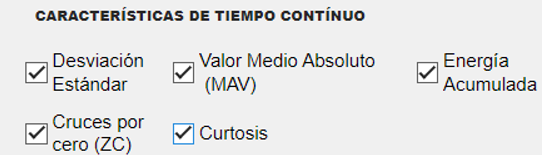
\includegraphics[width=0.4\textwidth]{figuras/26_carac_tiempo.png}
    \caption{Características en el dominio del tiempo continuo.}
    \label{fig: carac_tiempo}
\end{figure}

\begin{figure}[H]
    \centering
    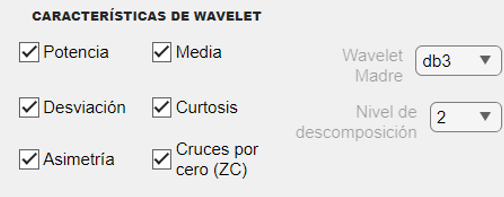
\includegraphics[width=0.4\textwidth]{figuras/27_carac_wavelet.png}
    \caption{Características con wavelets.}
    \label{fig: carac_wavelets}
\end{figure}

En cuanto a las características en el dominio de la frecuencia, la primera corrida se intento recolectar todas las características a la vez, como se puede observar en la Figura~\ref{fig: carac_freq}; pero el proceso se interrumpió al transcurrir las 6 horas y no finalizar. Por lo que se procedió a extraer las características una a la vez, obteniendo periodos de duración muy grandes en comparación a las características en el dominio del tiempo y wavelets. 

\begin{figure}[H]
    \centering
    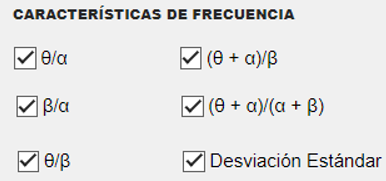
\includegraphics[width=0.4\textwidth]{figuras/28_carac_freq.png}
    \caption{Características en el dominio de la frecuencia.}
    \label{fig: carac_freq}
\end{figure}

\begin{table}[H]
\begin{center}
\begin{tabular}{|l|l|l|l|l|}
\hline
        \multicolumn{1}{|c|}{\textbf{Tipo}} &
   \textbf{ Hora inicio} & \textbf{Hora fin} & \textbf{Duración}\\ %\hline
          & (hh:mm:ss)  & (hh:mm:ss) & (hh:mm:ss)\\ \hline
    Tiempo continuo     & 14:54:00  & 15:33:07 & 00:39:07   \\ \hline
    Wavelet             & 15:35:00  & 15:35:32 & 00:00:32   \\ \hline
    Frecuencia          & 11:18:00  & 11:09:32 & 23:50:28   \\ \hline
    $\theta/\alpha$     & 17:10:25  & 18:26:52 & 01:16:27   \\ \hline
    $\beta/\alpha $     & 18:30:00  & 19:34:27 & 01:04:27   \\ \hline
    $\theta/\beta $     & 19:38:00  & 20:44:07 & 01:06:07   \\ \hline
\end{tabular}
\caption[Tiempos de extracción de características]{Tiempos de extracción de características con señales de HUMANA y UVG.} 
\label{cuadro:Duracion caracteristicas}
\end{center}
\end{table}

\section{Anotaciones automáticas}
El espacio de anotaciones automáticas necesita ser cargado con un set de datos provenientes de una señal bioeléctrica; un clasificador el cuál es el encargado de segmentar y así poder diferenciar el tipo de estado en el que se encuentra el paciente (Sano, ictal, preictal, interictal) y posteriormente se debe seleccionar los canales a analizar, como se observa en la Figura~\ref{fig: pre_anotaciones_ventana}. 

\begin{figure}[H]
    \centering
    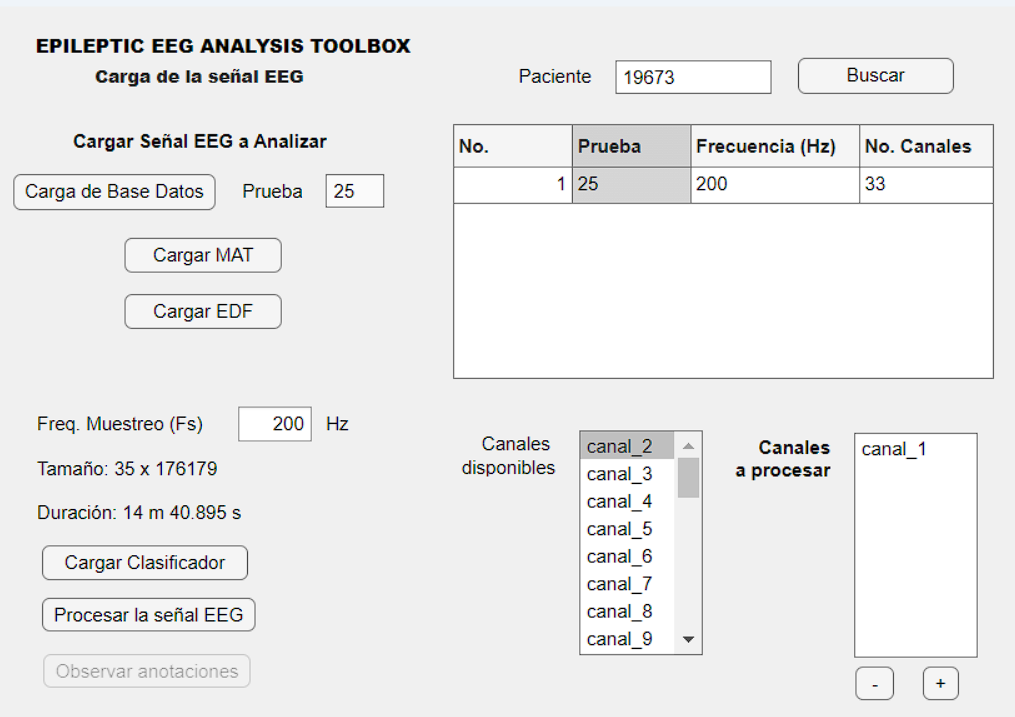
\includegraphics[width=0.6\textwidth]{figuras/31_ventana_preAnotaciones.png}
    \caption{Ventana de inicio para generar anotaciones automáticas.}
    \label{fig: pre_anotaciones_ventana}
\end{figure}

Para lo que se procedió a comprobar los tiempos de anotación según el clasificador, como se aprecia en el Cuadro~\ref{cuadro:Duracion anotaciones}. Como se puede observar nuevamente las wavelets son las características de menos duración, en este caso para la generación de anotaciones. 

\begin{table}[H]
\begin{center}
\begin{tabular}{|l|l|l|l|l|}
\hline
    \multicolumn{1}{|c|}{\textbf{Clasificador}} & \multicolumn{1}{c|}{\textbf{Duración }} & \multicolumn{1}{c|}{\textbf{Grabación }} \\ %\hline
          & (hh:mm:ss) & \\ \hline
    RNA Tiempo   & 01:27:00  & AL.edf   \\ \hline
    RNA Frecuencia& 01:07:00  & AL.edf   \\ \hline
    RNA Wavelet   & 00:12:00  & AL.edf   \\ \hline
\end{tabular}
\caption[Tiempos de entrenamiento para clasificadores]{Tiempos de entrenamiento para clasificadores con señales bioeléctricas de HUMANA y UVG.} 
\label{cuadro:Duracion anotaciones}
\end{center}
\end{table}

En las Figuras~\ref{fig: 33_chn_grafica} y \ref{fig: 33_chn_grafica_menos}, se observa la misma grabación brindada por HUMANA, la cual trata de una persona que tuvo iteradas ocasiones episodios epilépticos. La razón por la que visualmente difiere una de la otra es debido a la clasificación realizada, de lo cual se habla en los párrafos siguientes. 

En la grabación de las Figuras~\ref{fig: 33_chn_grafica} y \ref{fig: 33_chn_grafica_menos}, se percibe cambios abruptos, lo cual permite una diferencia visual de segmentos. Los segmento donde se encuentra una mayor densidad de oscilaciones y altas amplitudes (visualmente segmento más grueso), se debe a disparos de actividad bioeléctrica en el cerebro más movimiento físico debido a una convulsión. En cuanto a los segmento donde se percibe menos oscilaciones a una baja amplitud, son segmentos donde la persona no se encuentra en actividad ictal.  

Es en esta parte donde se puede notar la necesidad de una mayor cantidad de señales bioeléctricas por parte de HUMANA, ya que en la Figura~\ref{fig: 33_chn_grafica}, se muestra el resultado para la generación de anotaciones automáticas. Es casi nulo a simple vista, los segmentos que marcan actividad ictal (color rojo) versus los segmentos en estado sano (color azul). Esto en gran medida se debe a un fuerte sesgo de una mayor cantidad de datos EEG de personas sanas, que de personas con episodios epilépticos. 

\begin{figure}[H]
    \centering
    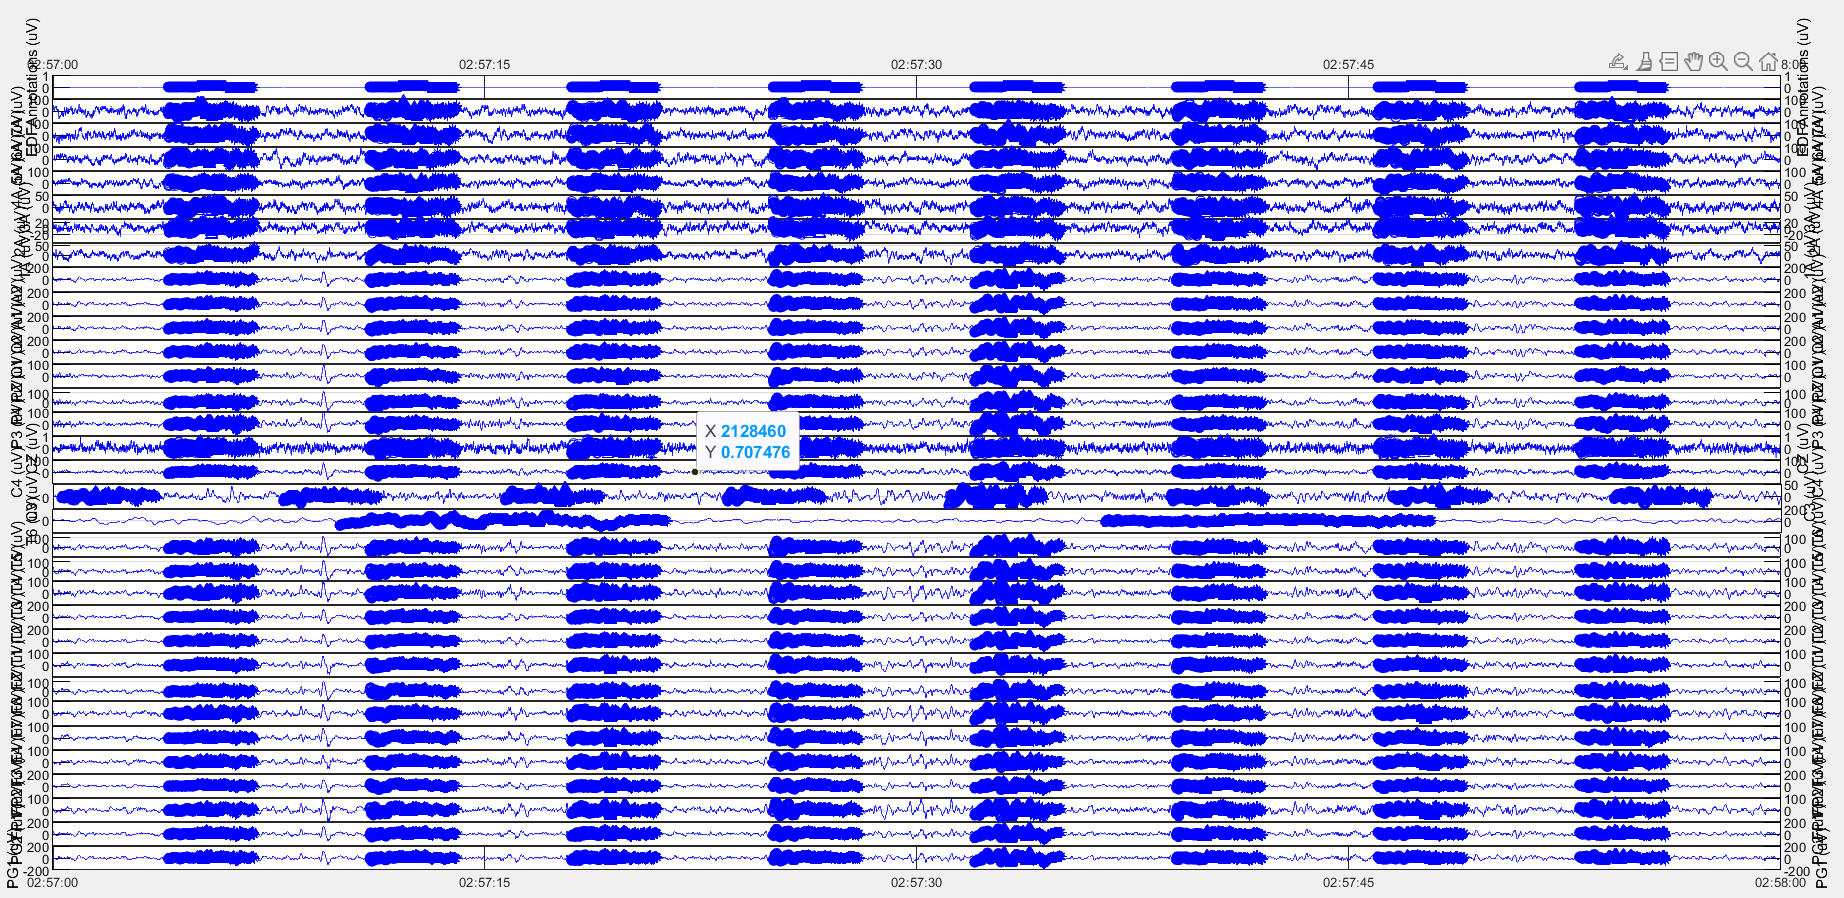
\includegraphics[width=0.77\textwidth]{figuras/30_33_canales_edf_humana.png}
    \caption{Anotaciones automáticas de 33 canales analizados.}
    \label{fig: 33_chn_grafica}
\end{figure}

Para solventar el inconveniente anterior sin contar con más datos por parte de HUMANA, se entreno al modelo con una menor cantidad de datos de personas sin actividad epiléptica. Desafortunadamente el resultado no fue el esperado. Como se puede observar en la Figura~\ref{fig: 33_chn_grafica_menos}, ahora se contaba con el inconveniente que era mayor el sesgo por los datos de actividad epiléptica respecto a los segmentos en estado sano.

\begin{figure}[H]
    \centering
    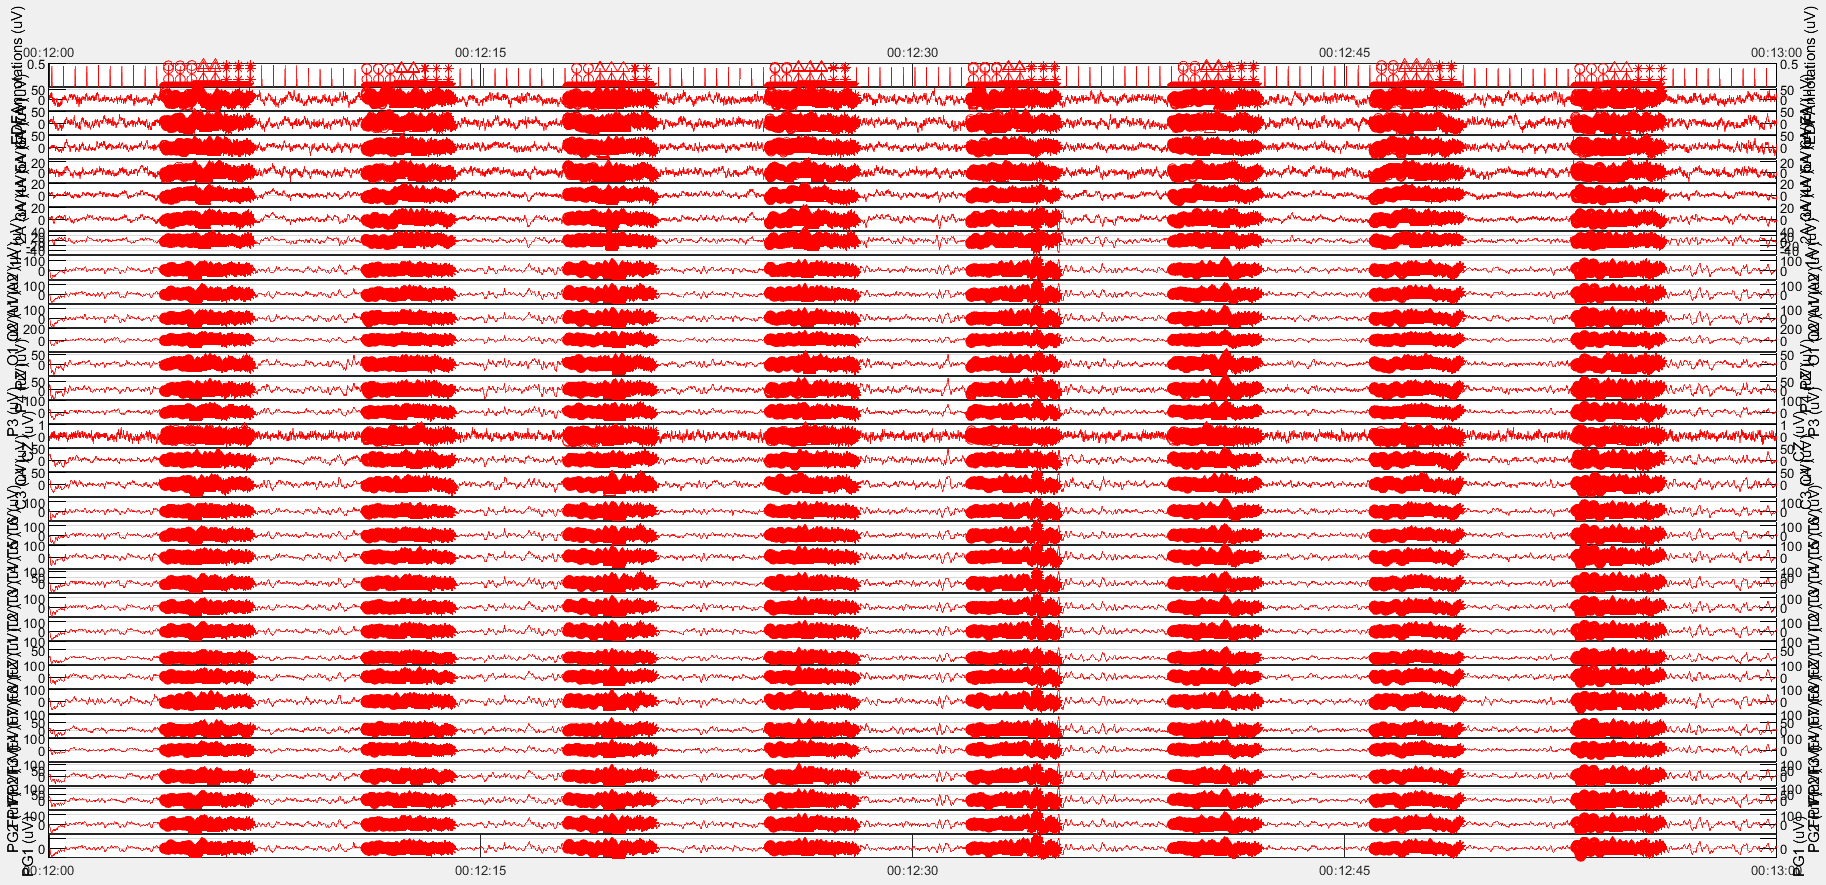
\includegraphics[width=0.77\textwidth]{figuras/33_33_canales_wavelet_edf_humana.png}
    \caption{Anotaciones automáticas de 33 canales analizados con menor cantidad de EEG de personas sin actividad ictal.}
    \label{fig: 33_chn_grafica_menos}
\end{figure}

Para solucionar este inconveniente, lo adecuado será entrenar el modelo con una cantidad similar de datos de señales bioeléctricas, además de, contar con la misma cantidad de personas sanas y personas con episodios epilépticos de las que se extraen las señales bioeléctricas. Esto permitirá al modelo encontrar las características necesarias de cada estado de interés, sin importar el sujeto. Ya que actualmente el modelo es preciso solo con las mismas personas con las que se entreno el modelo. Esto quiere decir que la predicción del modelo se ve afectada si, las señales bioeléctricas provienen de personas distintas de las que se obtuvieron los datos con los que se entrenó el modelo. 

\chapter{Resultados estadísticos}
En este capítulo, se presentan los resultados estadísticos obtenidos a partir de la aplicación de diversos métodos de análisis en el estudio de las señales bioeléctricas. Se analizan los resultados de los clasificadores empleados, se presentan las \gls{matrices de confusión} que reflejan la capacidad de predicción, y se evalúan los resultados de los algoritmos de \textit{clustering} mediante el algoritmo \textit{rand index}.

\section{Clasificadores}
Los clasificadores empleados para esta etapa mediante aprendizaje supervisado fueron las \gls{RNA}y las \gls{SVM}, dando resultados positivos. 

Las SVM presentaron una mejor clasificación de los segmentos de las  señales bioeléctricas, como se puede observar en las Figuras~\ref{fig: Matriz confusion svm wavelets}, \ref{fig: Matriz confusion svm time} y  \ref{fig: Matriz confusion svm freq}. Estando por encima de un 85\% de exactitud. Presentando que las características de mejor comportamiento para clasificación son las  ``wavelets'' seguidas de las características de ``tiempo continuo'' y por ultimo las características de ``frecuencia''.

Las RNA por su parte, también produjeron resultados positivos con ligera diferencia respecto a las SVM, como se puede observar en las Figuras~\ref{fig: Matriz confusion RNA wavelet}, \ref{fig: Matriz confusion RNA tiempo} y \ref{fig: Matriz confusion RNA freq}. Las cuales también se encuentran por encima del 85\% de exactitud. Se percibe nuevamente que las mejores características para la clasificación de señales bioeléctricas son ``wavelets'', en cuanto a las  características de ``tiempo continuo'' se nota una perdida del 0.4\% de exactitud respecto a la clasificación por SVM y una perdida del 0.2\% de exactitud empleando las características de ``frecuencia'' respecto a la clasificación por SVM.

\begin{figure}[H]
    \centering
    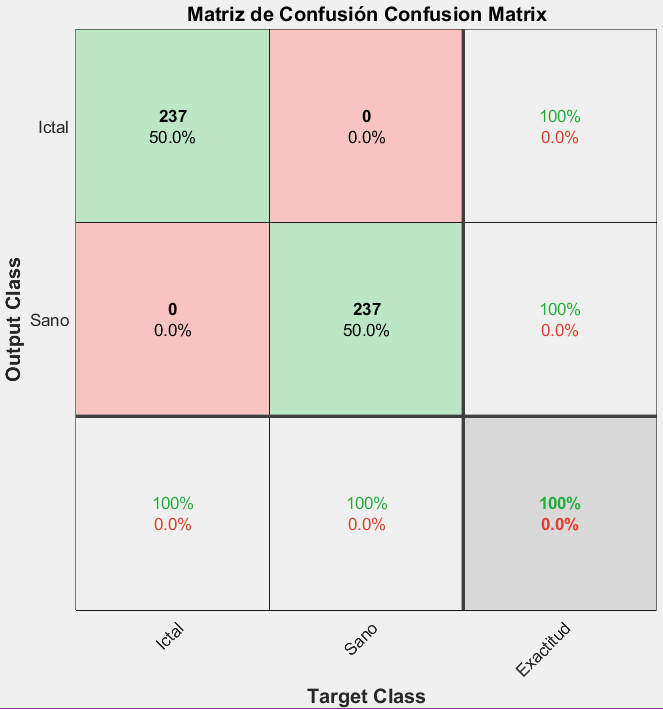
\includegraphics[width=0.5\textwidth]{figuras/37_svm_wavelet_edf_15ubon.png}
    \caption{Matriz de confusión para las clases Ictal y Sano utilizando SVM con características wavelets.}
    \label{fig: Matriz confusion svm wavelets}
\end{figure}
\begin{figure}[H]
    \centering
    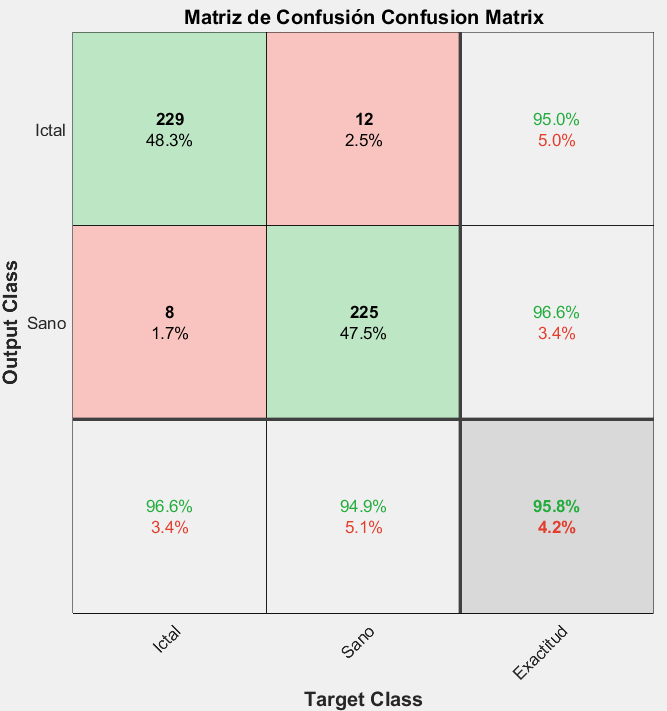
\includegraphics[width=0.5\textwidth]{figuras/38_svm_time_edf_15ubon.png}
    \caption{Matriz de confusión para las clases Ictal y Sano utilizando SVM con características en tiempo continuo.}
    \label{fig: Matriz confusion svm time}
\end{figure}
\begin{figure}[H]
    \centering
    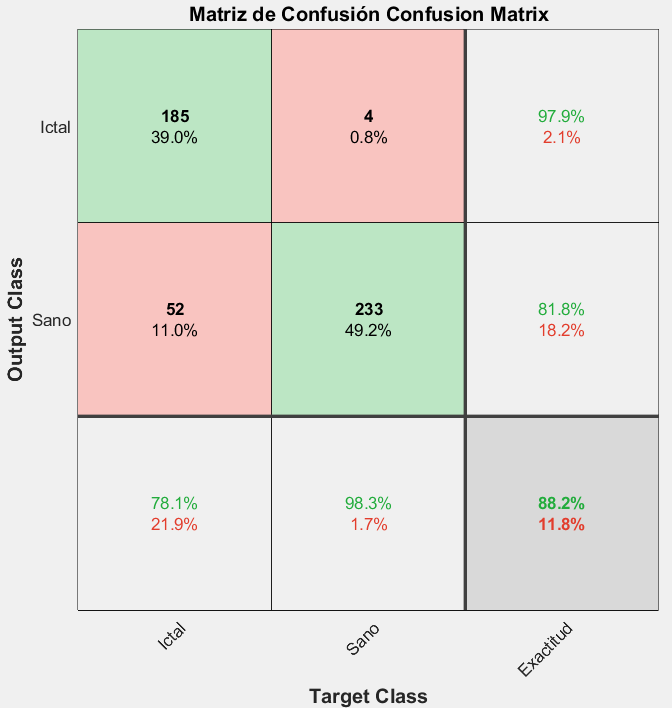
\includegraphics[width=0.5\textwidth]{figuras/36_svm_freq_edf_15ubon.png}
    \caption{Matriz de confusión para las clases Ictal y Sano utilizando SVM con características frecuencia.}
    \label{fig: Matriz confusion svm freq}
\end{figure}

\begin{figure}[H]
    \centering
    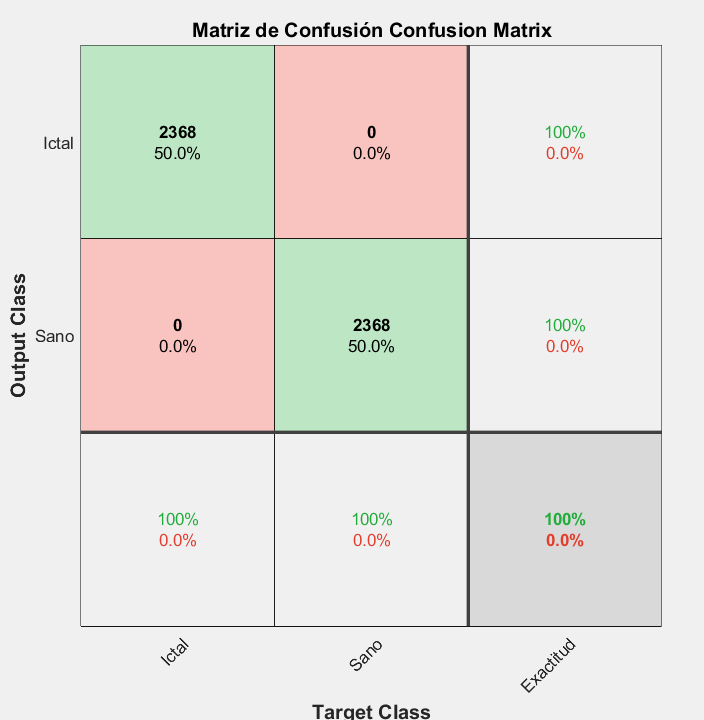
\includegraphics[width=0.5\textwidth]{figuras/32_rnn_wavelet_edf_15ubon.png}
    \caption{Matriz de confusión para las clases Ictal y Sano utilizando RNA con características wavelets.}
    \label{fig: Matriz confusion RNA wavelet}
\end{figure}
\begin{figure}[H]
    \centering
    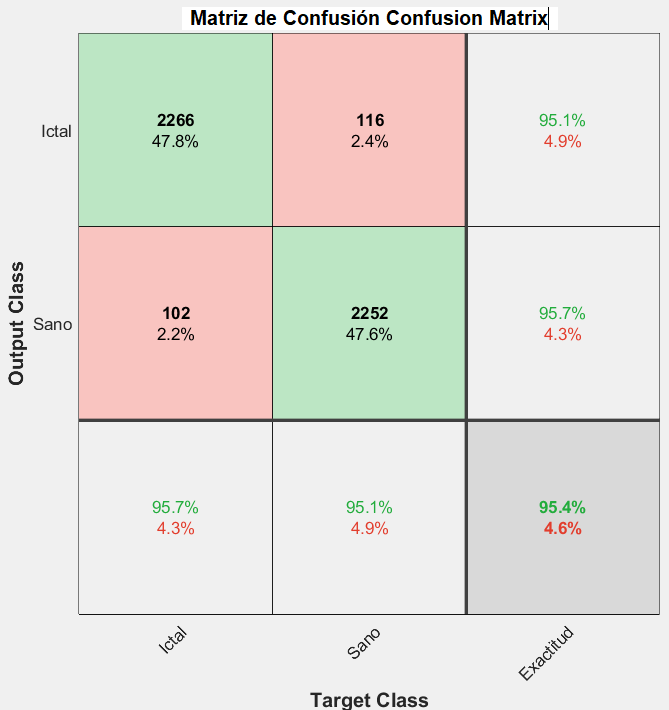
\includegraphics[width=0.5\textwidth]{figuras/34_rnn_tiempo_edf_15ubon.png}
    \caption{Matriz de confusión para las clases Ictal y Sano utilizando RNA con características en tiempo continuo.}
    \label{fig: Matriz confusion RNA tiempo}
\end{figure}
\begin{figure}[H]
    \centering
    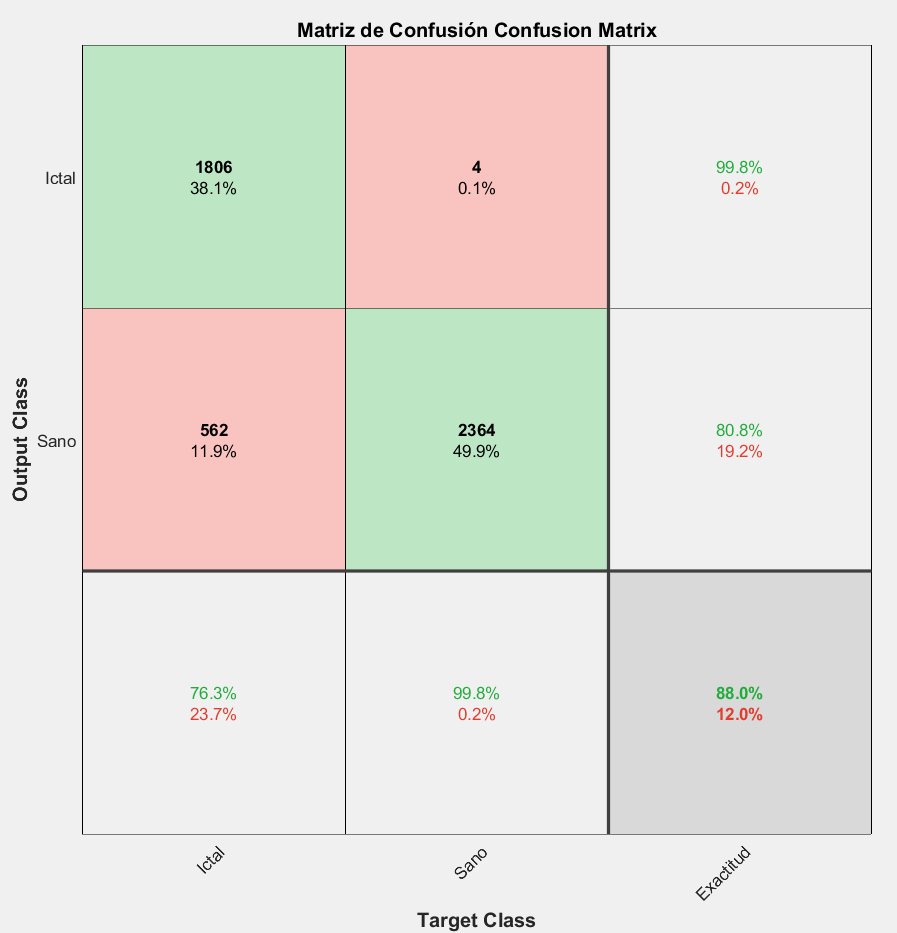
\includegraphics[width=0.55\textwidth]{figuras/35_rnn_freq_edf_15ubon.png}
    \caption{Matriz de confusión para las clases Ictal y Sano utilizando RNA con características en frecuencia.}
    \label{fig: Matriz confusion RNA freq}
\end{figure}

\section{Algoritmos de agrupamiento}
Los algoritmos de agrupamiento empleados para esta etapa mediante aprendizaje no supervisado fueron \textit{K-means} y jerárquico, obteniendo resultados positivos. 

Como se puede observar en el Cuadro~\ref{cuadro:resultado rand index}, las características ``wavelets'' y ``tiempo continuo'' independientemente del algoritmo de agrupación se obtienen los mismos resultados, sin embargo, para  las características de ``frecuencia'' si se nota una gran mejora de clasificación con el algoritmo de agrupamiento jerárquico dando un 30.46\% de superioridad versus el algoritmo de agrupamiento \textit{K-means}.

Por lo que nuevamente las características ``wavelets'' son las que presentan mejores resultado para la clasificación de segmentos de interés en señales bioeléctricas. Para las características en ``tiempo continuo'' se puede mejorar el porcentaje de clasificación obteniendo una mayor cantidad de características. En cuanto a las características de ``frecuencia'' si es notorio una mejora para el algoritmo de agrupamiento jerárquico. Las características en el dominio de la frecuencia a menudo tienen una estructura más jerárquica y pueden exhibir patrones de similitud a diferentes escalas. El agrupamiento jerárquico se adapta bien a la estructura jerárquica de los datos y puede identificar grupos en diferentes niveles de detalle, lo que puede ser beneficioso en datos con patrones complejos.

\begin{table}[H]
\begin{center}
    \begin{tabular}{|l|l|r|}
    \hline
        \multicolumn{1}{|c|}{\textbf{Algoritmo de agrupamiento}} & \multicolumn{1}{c|}{\textbf{Característica}} & \multicolumn{1}{c|}{\textbf{Rand index}}\\ \hline
        K-means  & Wavelets &  100.00\% \\ \hline
        K-means  & Tiempo continuo & 70.68\% \\ \hline
        K-means  & Frecuencia & 50.01\% \\ \hline
        Jerárquico & Wavelets &  100.00\% \\ \hline
        Jerárquico & Tiempo continuo & 70.68\% \\ \hline
        Jerárquico & Frecuencia & 91.55\% \\ \hline
    \end{tabular}
    \caption[Resultado rand index para algoritmos de agrupamiento]{Porcentaje de validación para los algoritmos de agrupamiento mediante \textit{rand index}.} 
    \label{cuadro:resultado rand index}
\end{center}
\end{table}

\chapter{Análisis de grupos}
El análisis de grupos (\textit{clustering}) desempeña un papel fundamental en la investigación, ya que permite explorar la estructura subyacente de las señales bioeléctricas recopiladas. En este capítulo, se presentan los resultados del uso de algoritmos de agrupamiento, en particular el método de K-means y jerárquico, aplicados a las señales bioeléctricas en diferentes dominios: tiempo, frecuencia y wavelets. Cabe mencionar que los datos utilizados son el resultado de una época de 0.4 segundos, por lo que la densidad de muestras cambiara según la frecuencia con la que se haya grabado la señal bioeléctrica para las clases ictal, sano, preictal e interictal.
%revisar app "generacionesalgoritmo.mlapp" linea 323, variable "app.s_ventana"

En el enfoque de análisis, se aplicó el método de \textit{clustering} utilizando todos las características extraídas de las señales bioeléctricas. La decisión de emplear el conjunto completo de características se basa en la premisa de que cada característica contribuye de manera única a la representación de la información en los datos. Utilizando todas las características, se busca capturar la complejidad y la variabilidad completa presente en las señales.

Posteriormente, para la visualización de los resultados, se graficaron pares específicos de características seleccionadas. Dada la naturaleza multidimensional de los datos, la representación gráfica de las características se limita a graficar pares específicos, ya que la visualización directa de espacios de características con más de tres dimensiones se vuelve inherentemente compleja. La elección de graficar pares específicos permite explorar las relaciones bidimensionales entre características seleccionadas, ofreciendo una perspectiva visual que facilita la interpretación de patrones y tendencias. A pesar de la limitación en la representación tridimensional, la estrategia de graficar pares específicos proporciona una visión detallada de las interacciones entre características, contribuyendo a la comprensión global de la estructura de los datos y respaldando el análisis de los resultados obtenidos mediante los algoritmos de \textit{clustering} aplicados al conjunto completo de características.

En la ultima sección de este capitulo se hablará acerca de la incorporación de la herramienta VAT, la cual ha resultado fundamental para abordar el desafío de visualizar las clases en un espacio multidimensional sin perder información relevante debido a la alta dimensionalidad de los datos. VAT proporciona una representación visual eficaz al reducir la complejidad de los datos, permitiendo la observación de patrones y relaciones entre clases. Esta herramienta ha facilitado la identificación de estructuras y la evaluación de la tendencia de agrupamiento en el conjunto de datos, mejorando así la comprensión y la interpretación de los resultados de los algoritmos de clustering aplicados en contextos de alta dimensionalidad.

\section{Análisis de Grupos en el Dominio de Tiempo}
En esta sección, se presenta el análisis de grupos aplicado a las características extraídas en el dominio del tiempo. 
Las características que se extrajeron en el dominio del tiempo fueron:
\begin{enumerate}
    \item Desviación estándar
    \item Valor medio absoluto (MAV)
    \item Cruces por cero (ZC)
    \item Curtosis
    \item Energía acumulada
\end{enumerate}

\subsection{Resultados K-means}

Los resultados del proceso de agrupamiento en el dominio de tiempo revelan una interesante distribución de los datos. En particular,como se observa en las Figuras~\ref{fig: k_means_Time_1_2} y \ref{fig: k_means_time_1_4} la distribución de los datos son muy continuos, lo cual indica que las características 1 respecto de 2 y 1 respecto de 4 podrían no ser muy efectivas para la predicción del tipo de señal bioeléctrica. Mientras que en las Figuras ~\ref{fig: k_means_time_1_5}, \ref{fig: k_means_time_2_4}, \ref{fig: k_means_time_2_5} y \ref{fig: k_means_time_4_5}. Los datos tienden a concentrarse de manera significativa en uno de los grupos, mientras que el otro grupo muestra una menor concentración de datos. 

La gran concentración de datos en un grupo y la menor concentración en el otro grupo indican que las señales bioeléctricas pueden categorizarse de manera efectiva en función de estas características en el dominio del tiempo. Esto sugiere la existencia de patrones distintivos que permiten la separación de las señales en dos grupos significativos. Aunque cabe destacar que es aquí donde se percibe la necesidad de una mayor cantidad de datos de pacientes con epilepsia, lo que permitiría tener dos grupos igual de densos en datos. 

\begin{figure}[H]
    \centering
    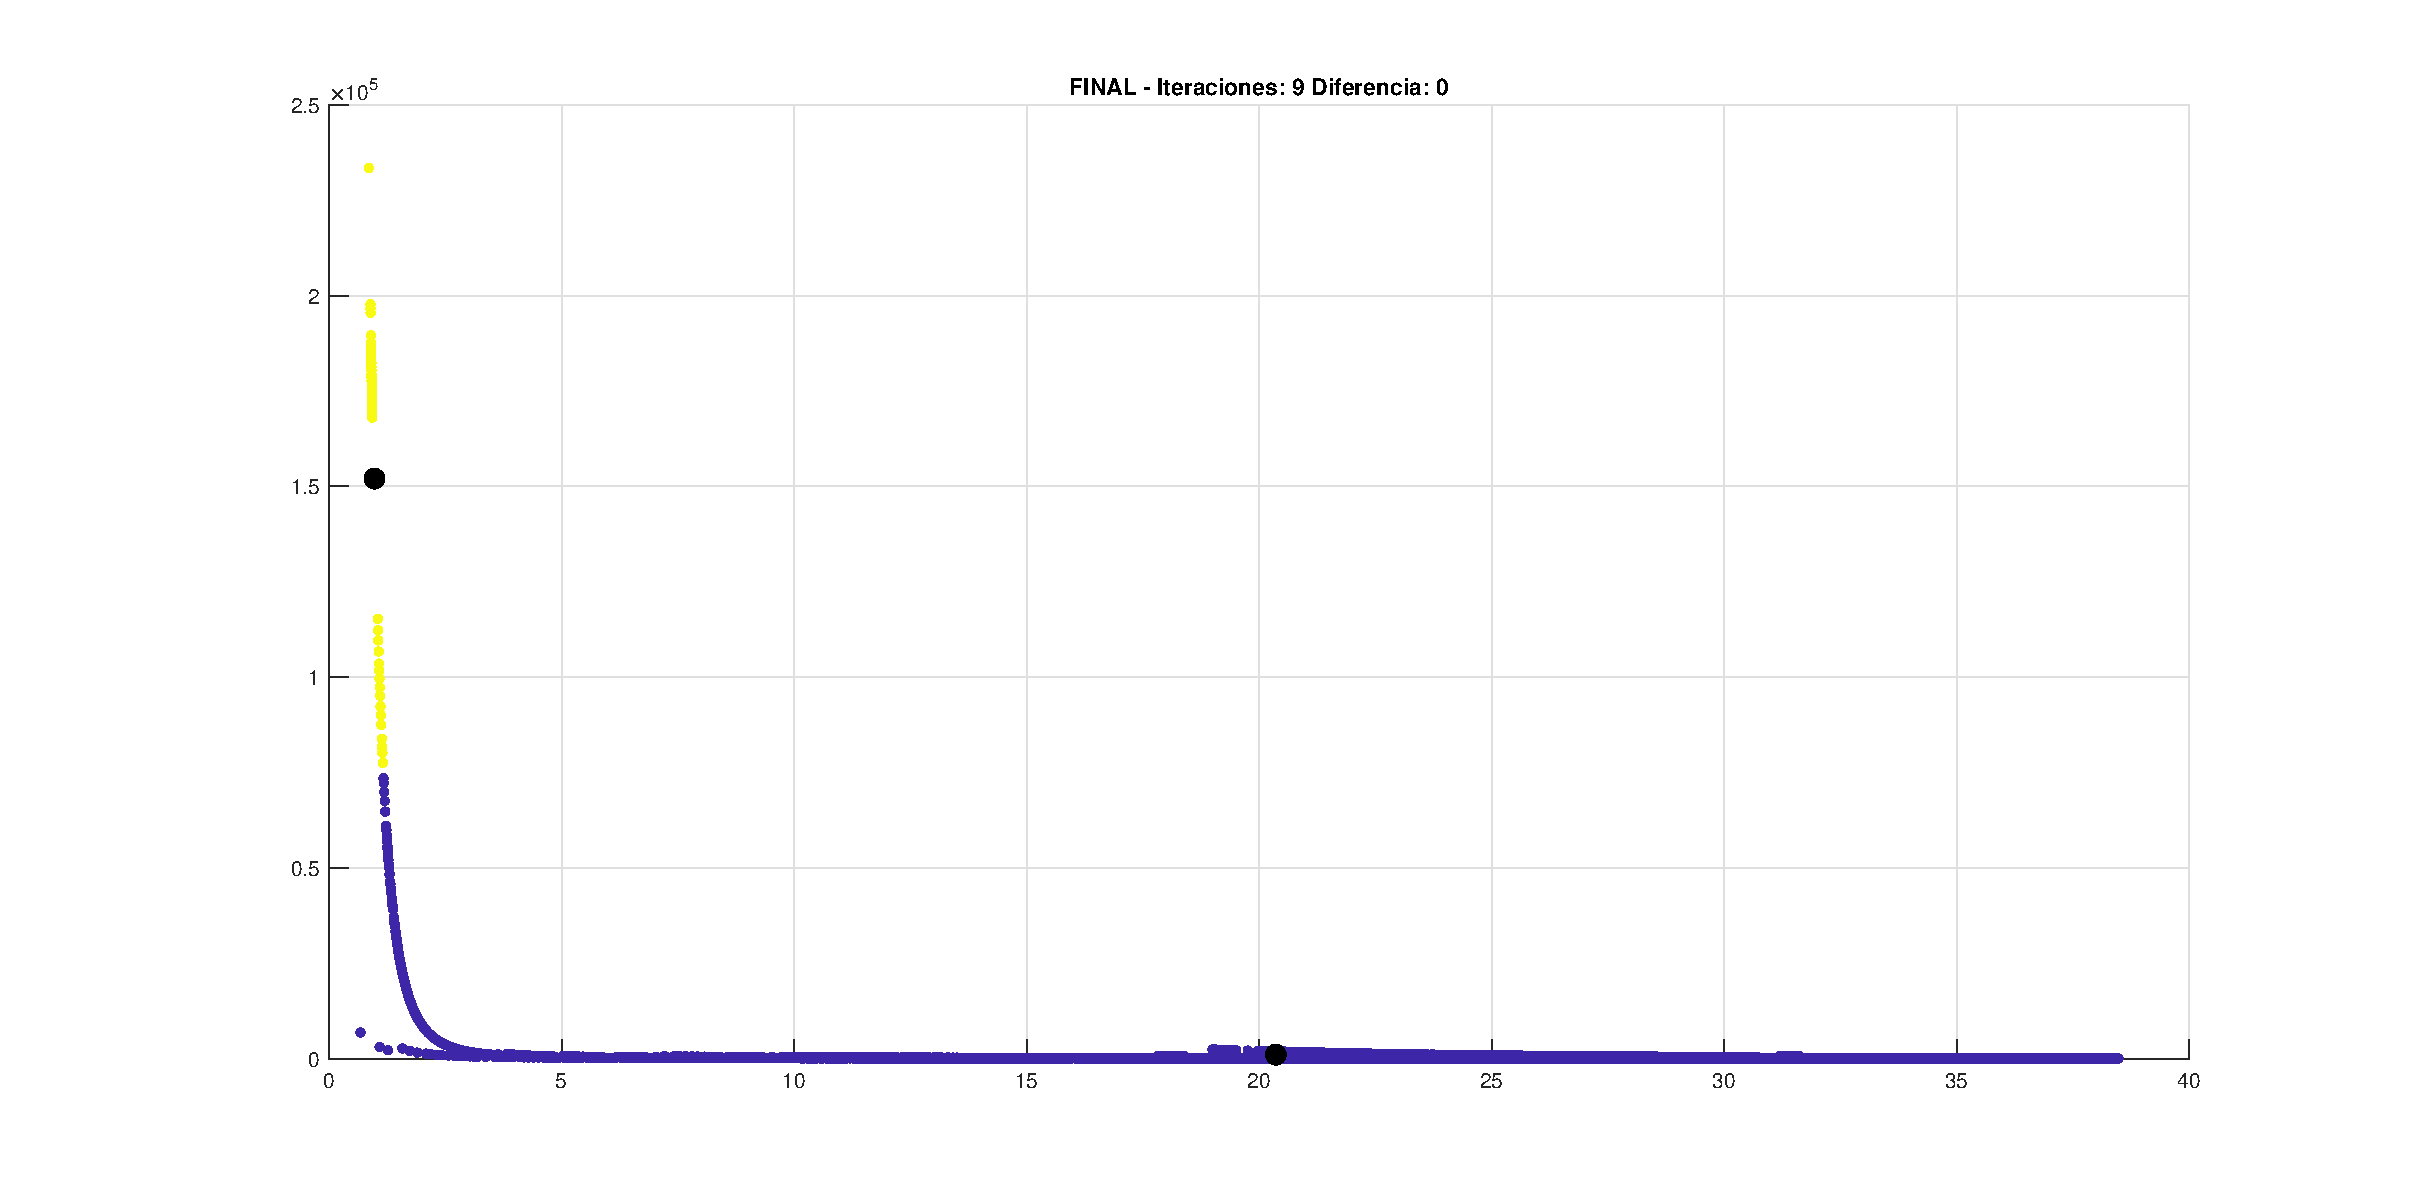
\includegraphics[width=0.90\textwidth]{figuras/k_means_time_1and2_sano_ictal.eps}
    \caption{Gráfica de agrupamiento por k-means de señales bioeléctricas de las características 1 y 2 en el dominio del tiempo  de actividad ictal y no ictal.}
    \label{fig: k_means_Time_1_2}
\end{figure}

\begin{figure}[H]
    \centering
    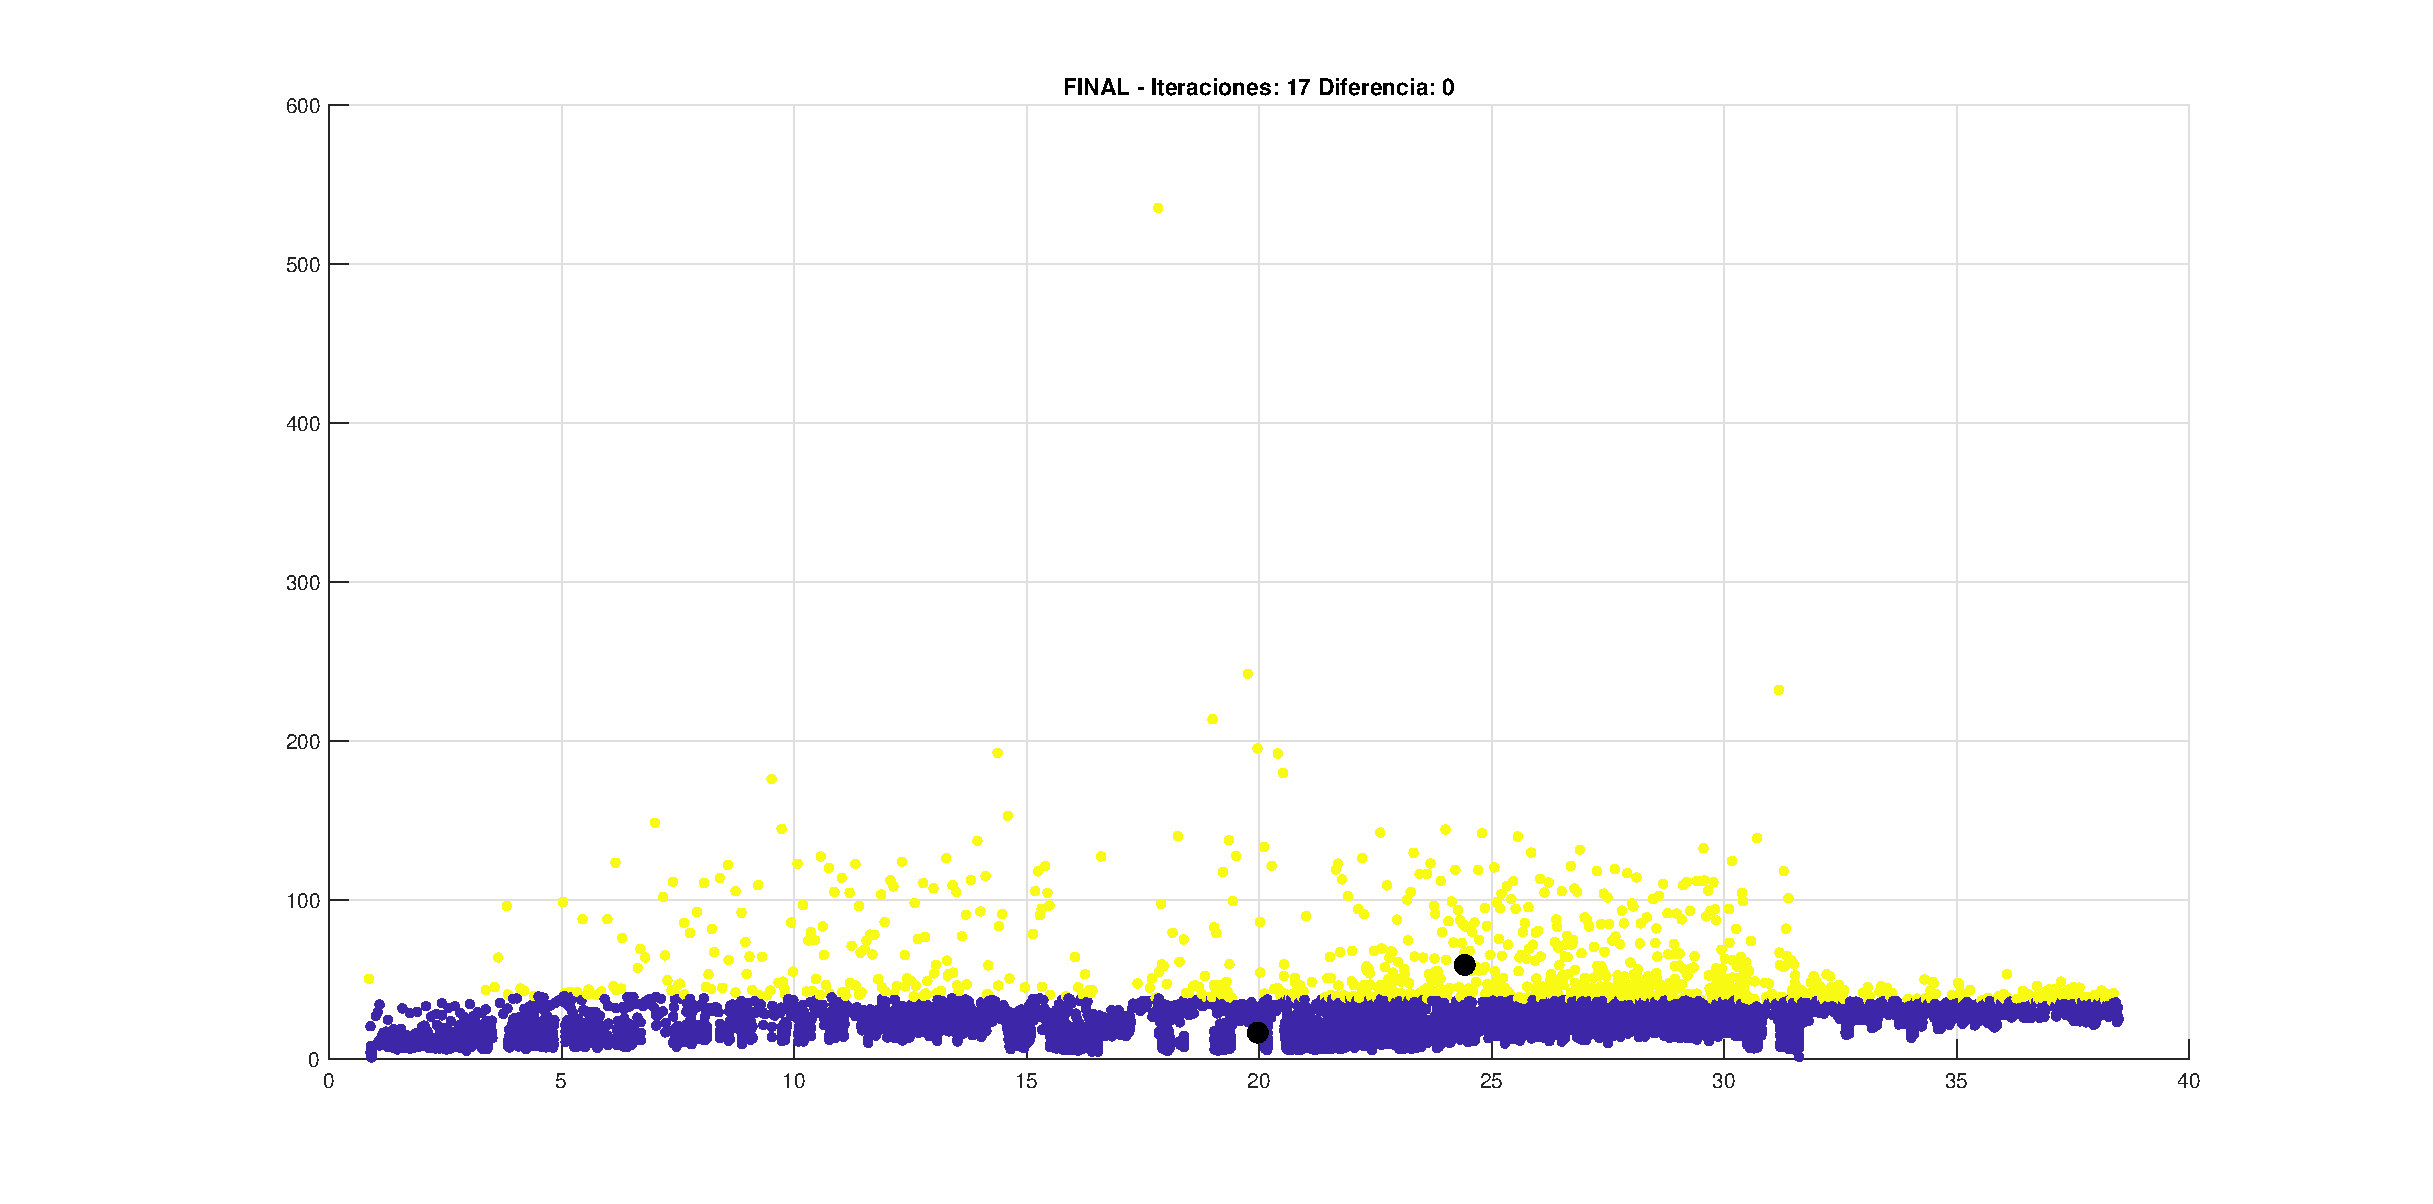
\includegraphics[width=0.90\textwidth]{figuras/k_means_time_1and4_sano_ictal.eps}
    \caption{Gráfica de agrupamiento por k-means de señales bioeléctricas de las características 1 y 4 en el dominio del tiempo de actividad ictal y no ictal.}
    \label{fig: k_means_time_1_4}
\end{figure}
\begin{figure}[H]
    \centering
    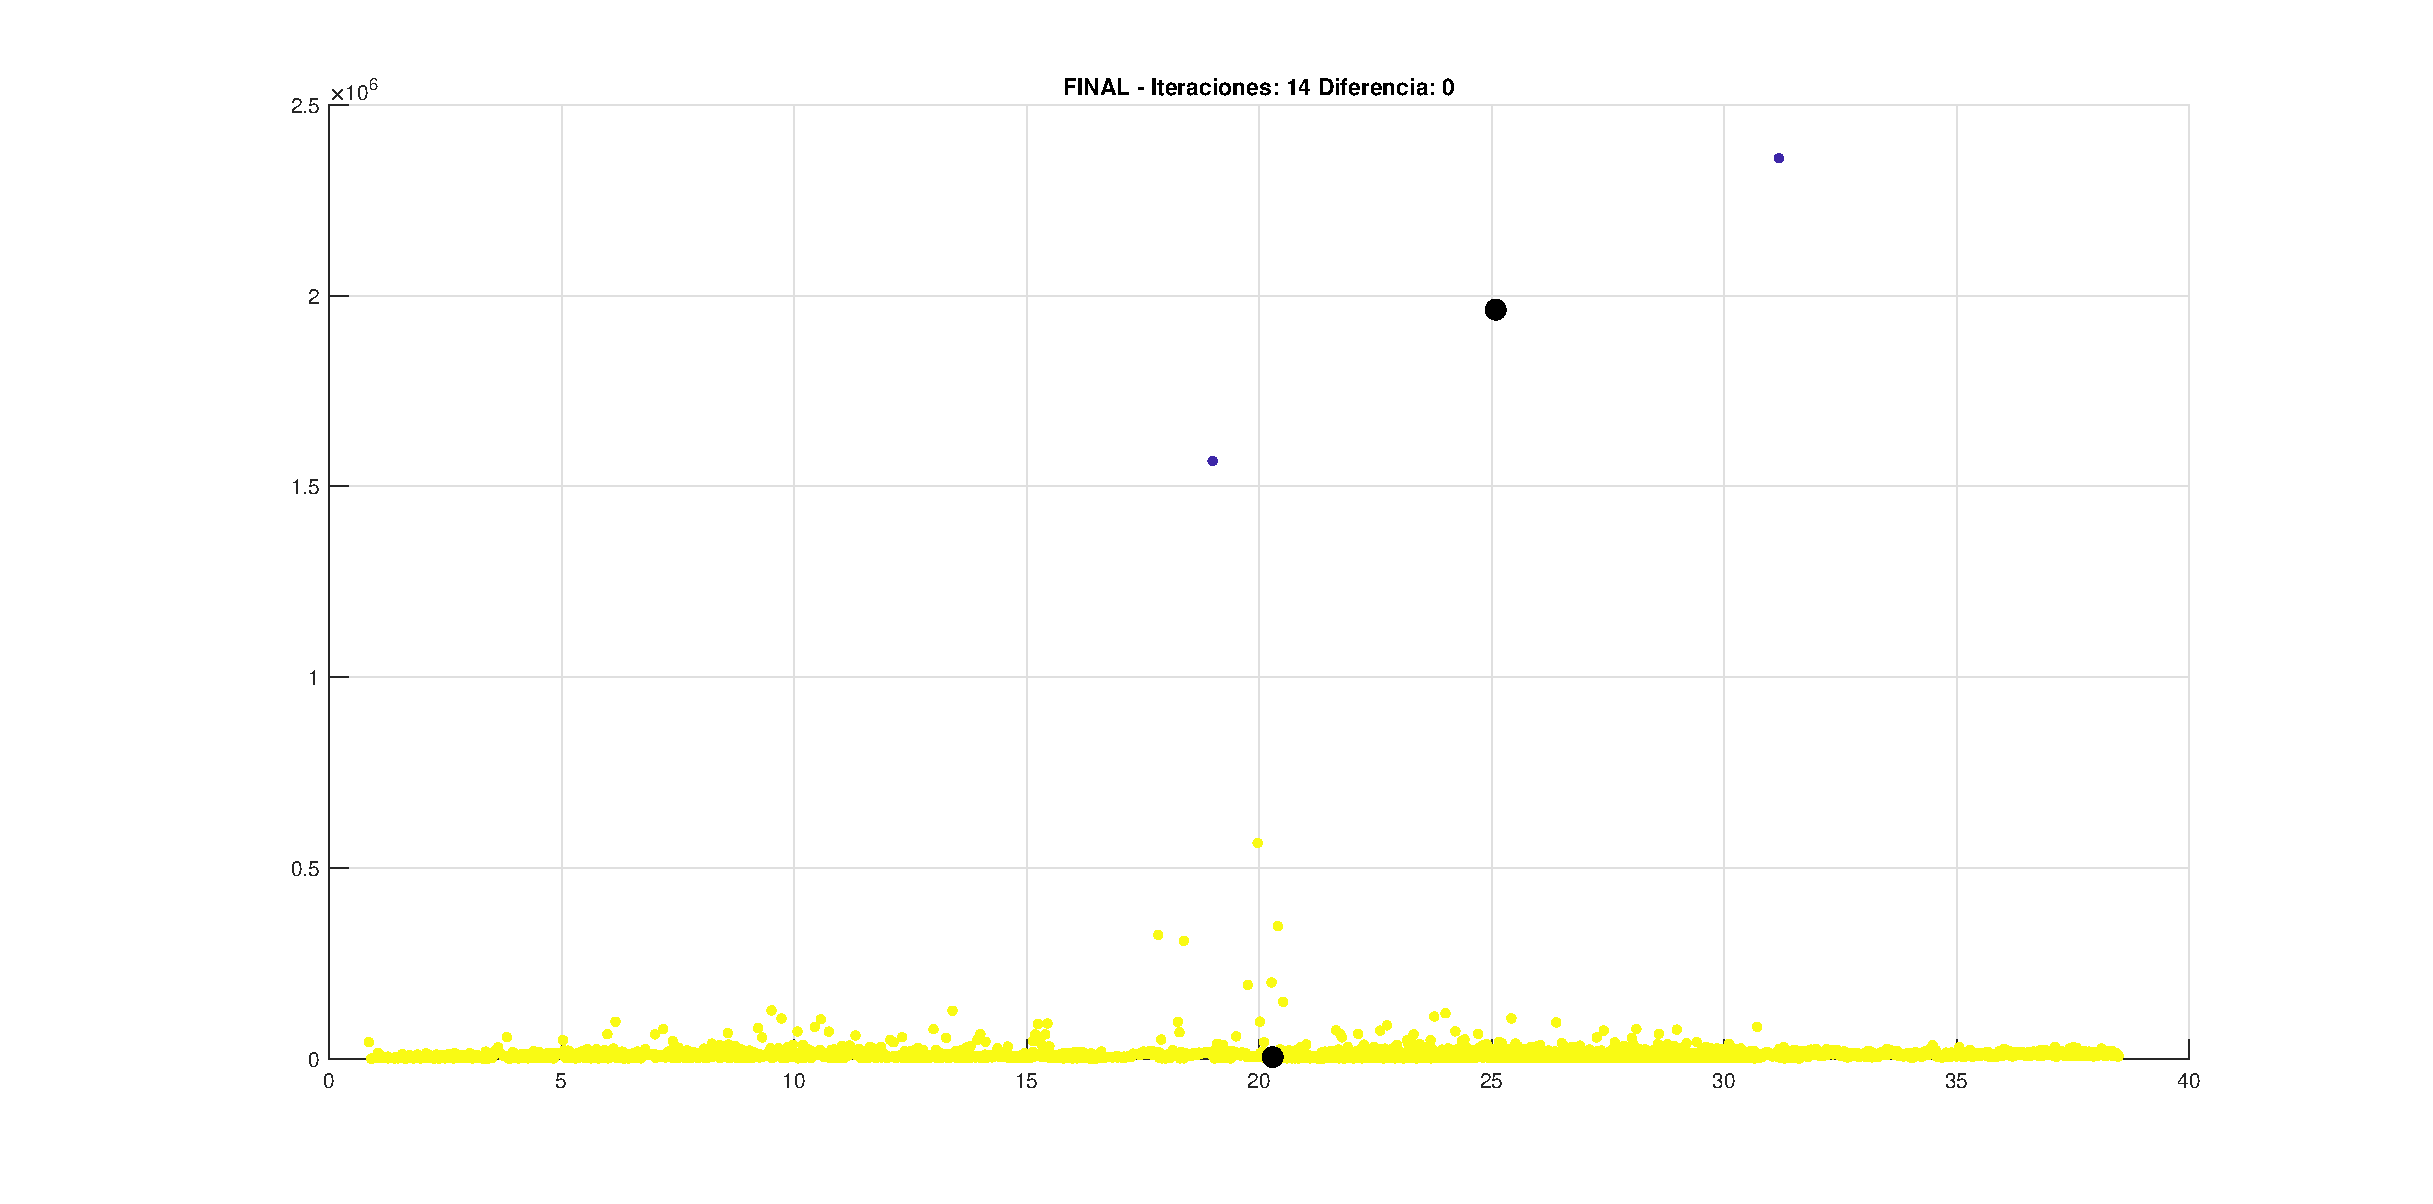
\includegraphics[width=0.90\textwidth]{figuras/k_means_time_1and5_sano_ictal.eps}
    \caption{Gráfica de agrupamiento por k-means de señales bioeléctricas de las características 1 y 5 en el dominio del tiempo de actividad ictal y no ictal.}
    \label{fig: k_means_time_1_5}
\end{figure}
\begin{figure}[H]
    \centering
    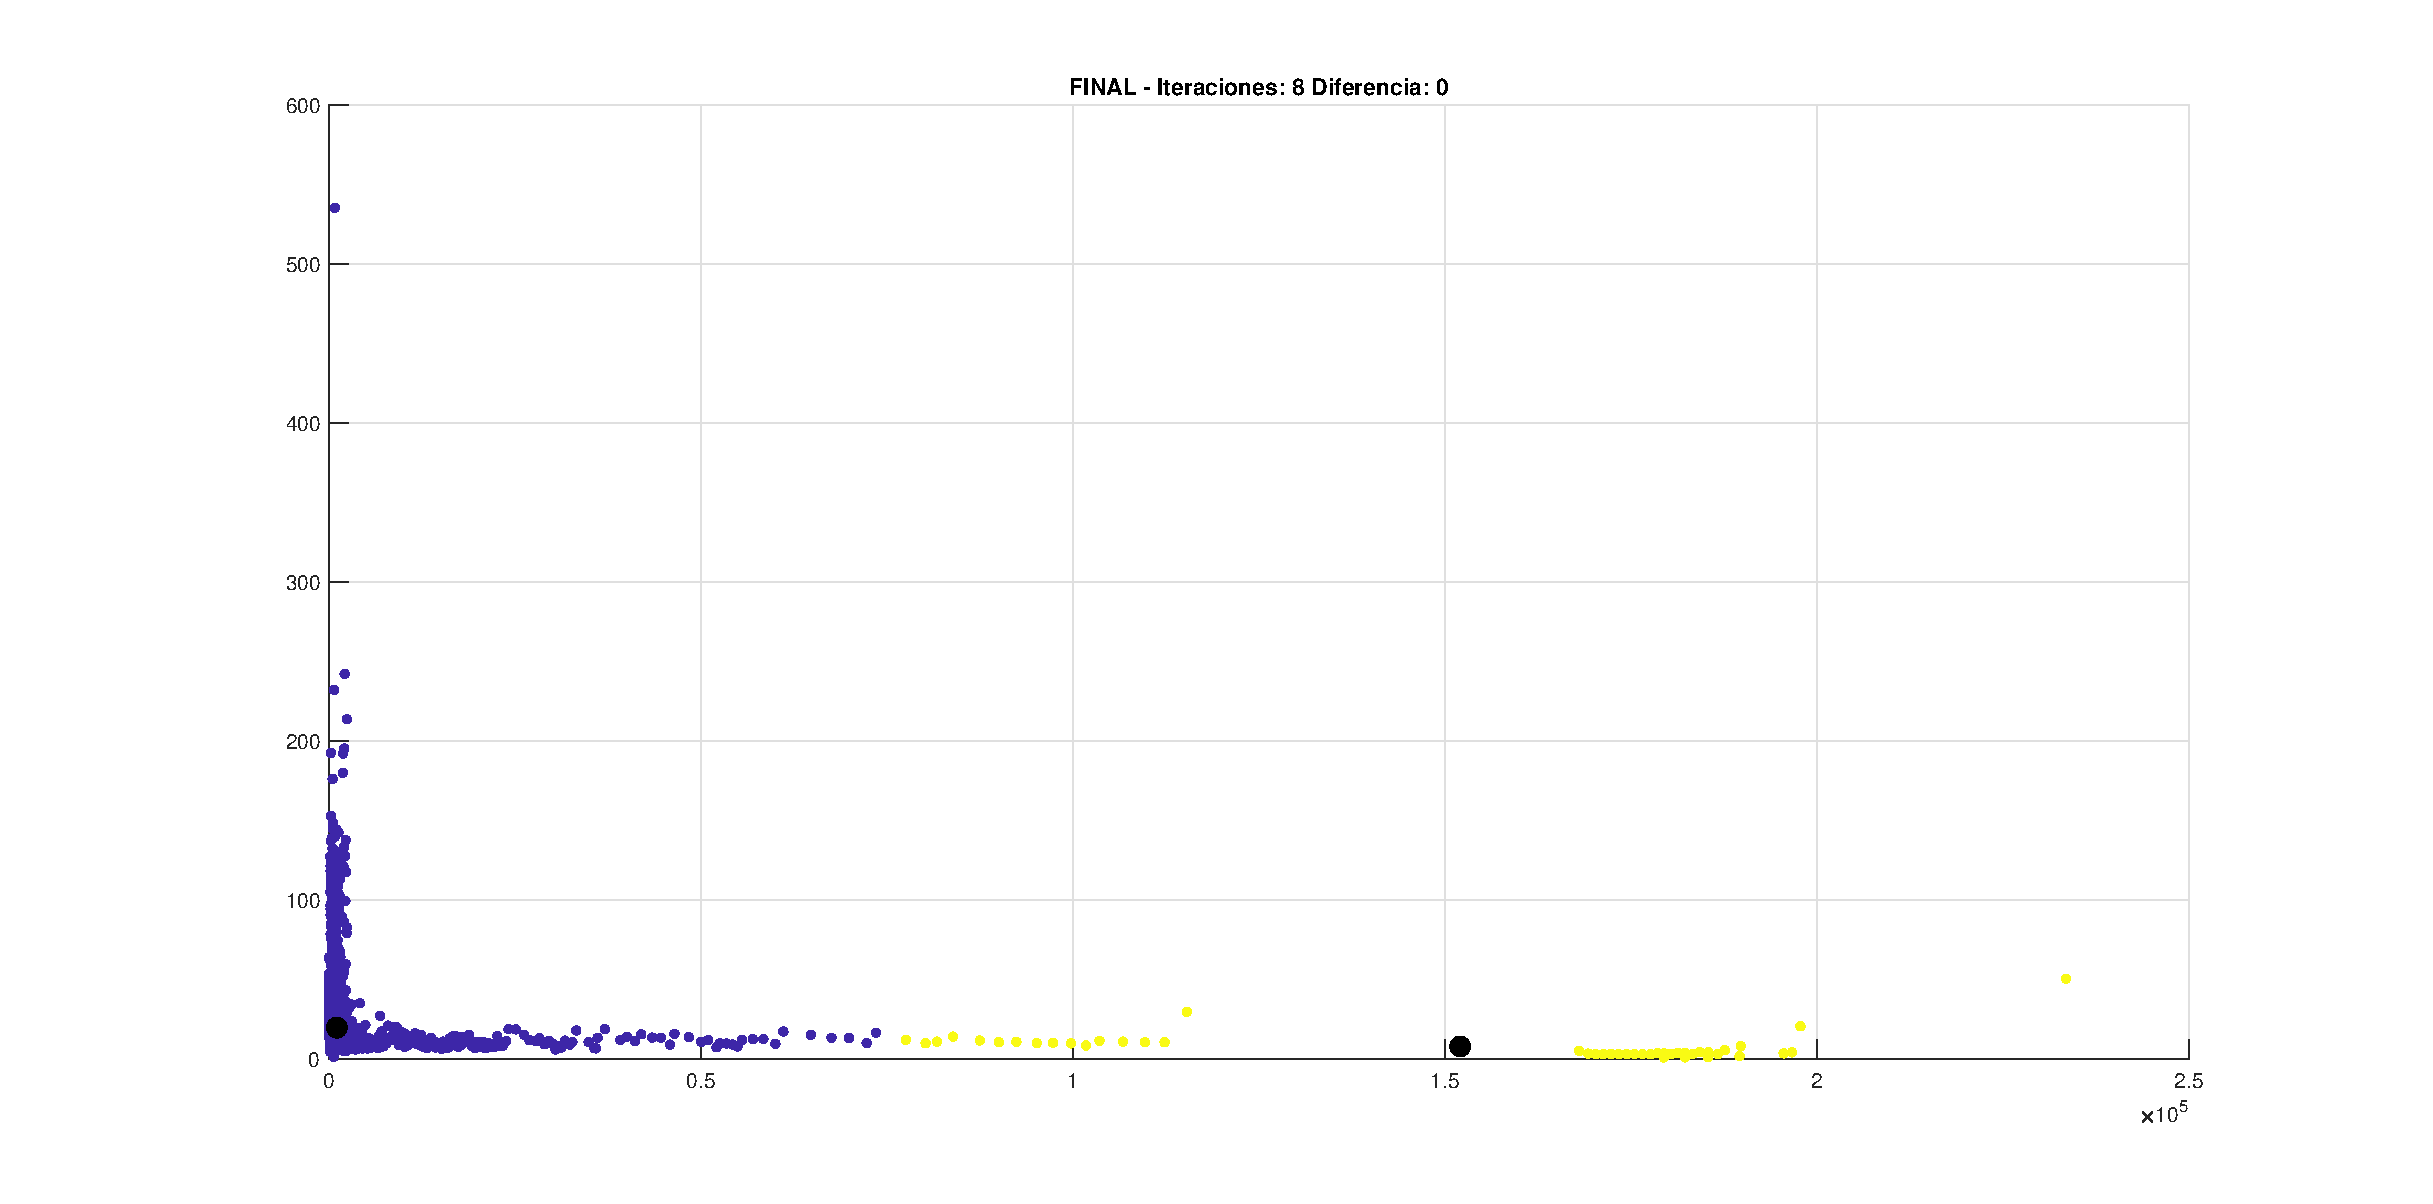
\includegraphics[width=0.90\textwidth]{figuras/k_means_time_2and4_sano_ictal.eps}
    \caption{Gráfica de agrupamiento por k-means de señales bioeléctricas de las características 2 y 4 en el dominio del tiempo de actividad ictal y no ictal.}
    \label{fig: k_means_time_2_4}
\end{figure}
\begin{figure}[H]
    \centering
    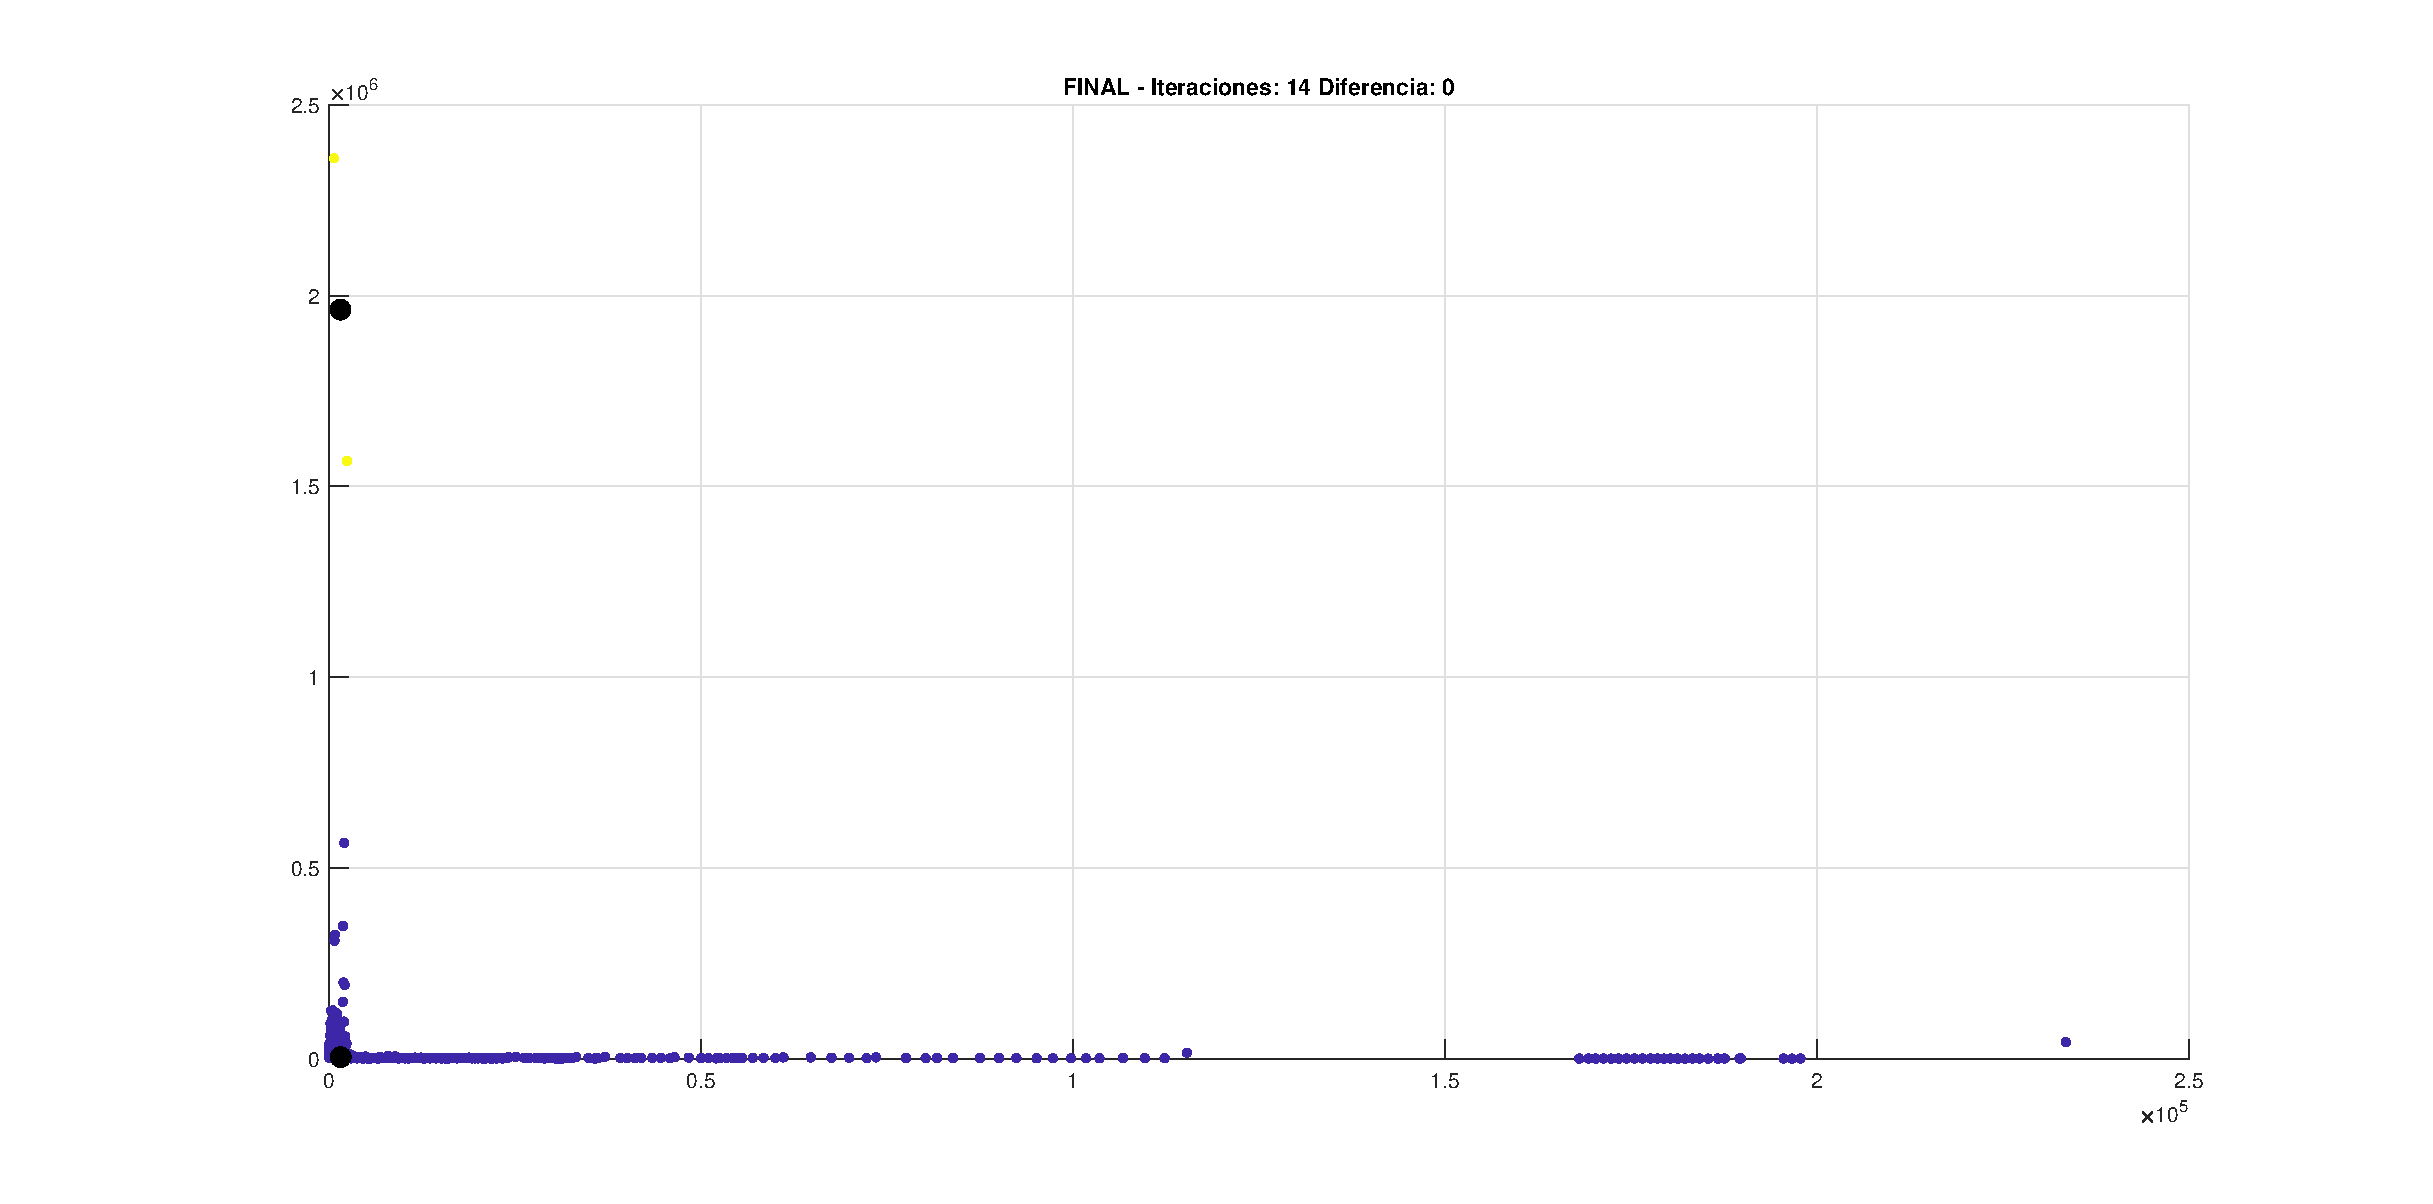
\includegraphics[width=0.90\textwidth]{figuras/k_means_time_2and5_sano_ictal.eps}
    \caption{Gráfica de agrupamiento por k-means de señales bioeléctricas de las características 2 y 5 en el dominio del tiempo de actividad ictal y no ictal.}
    \label{fig: k_means_time_2_5}
\end{figure}
\begin{figure}[H]
    \centering
    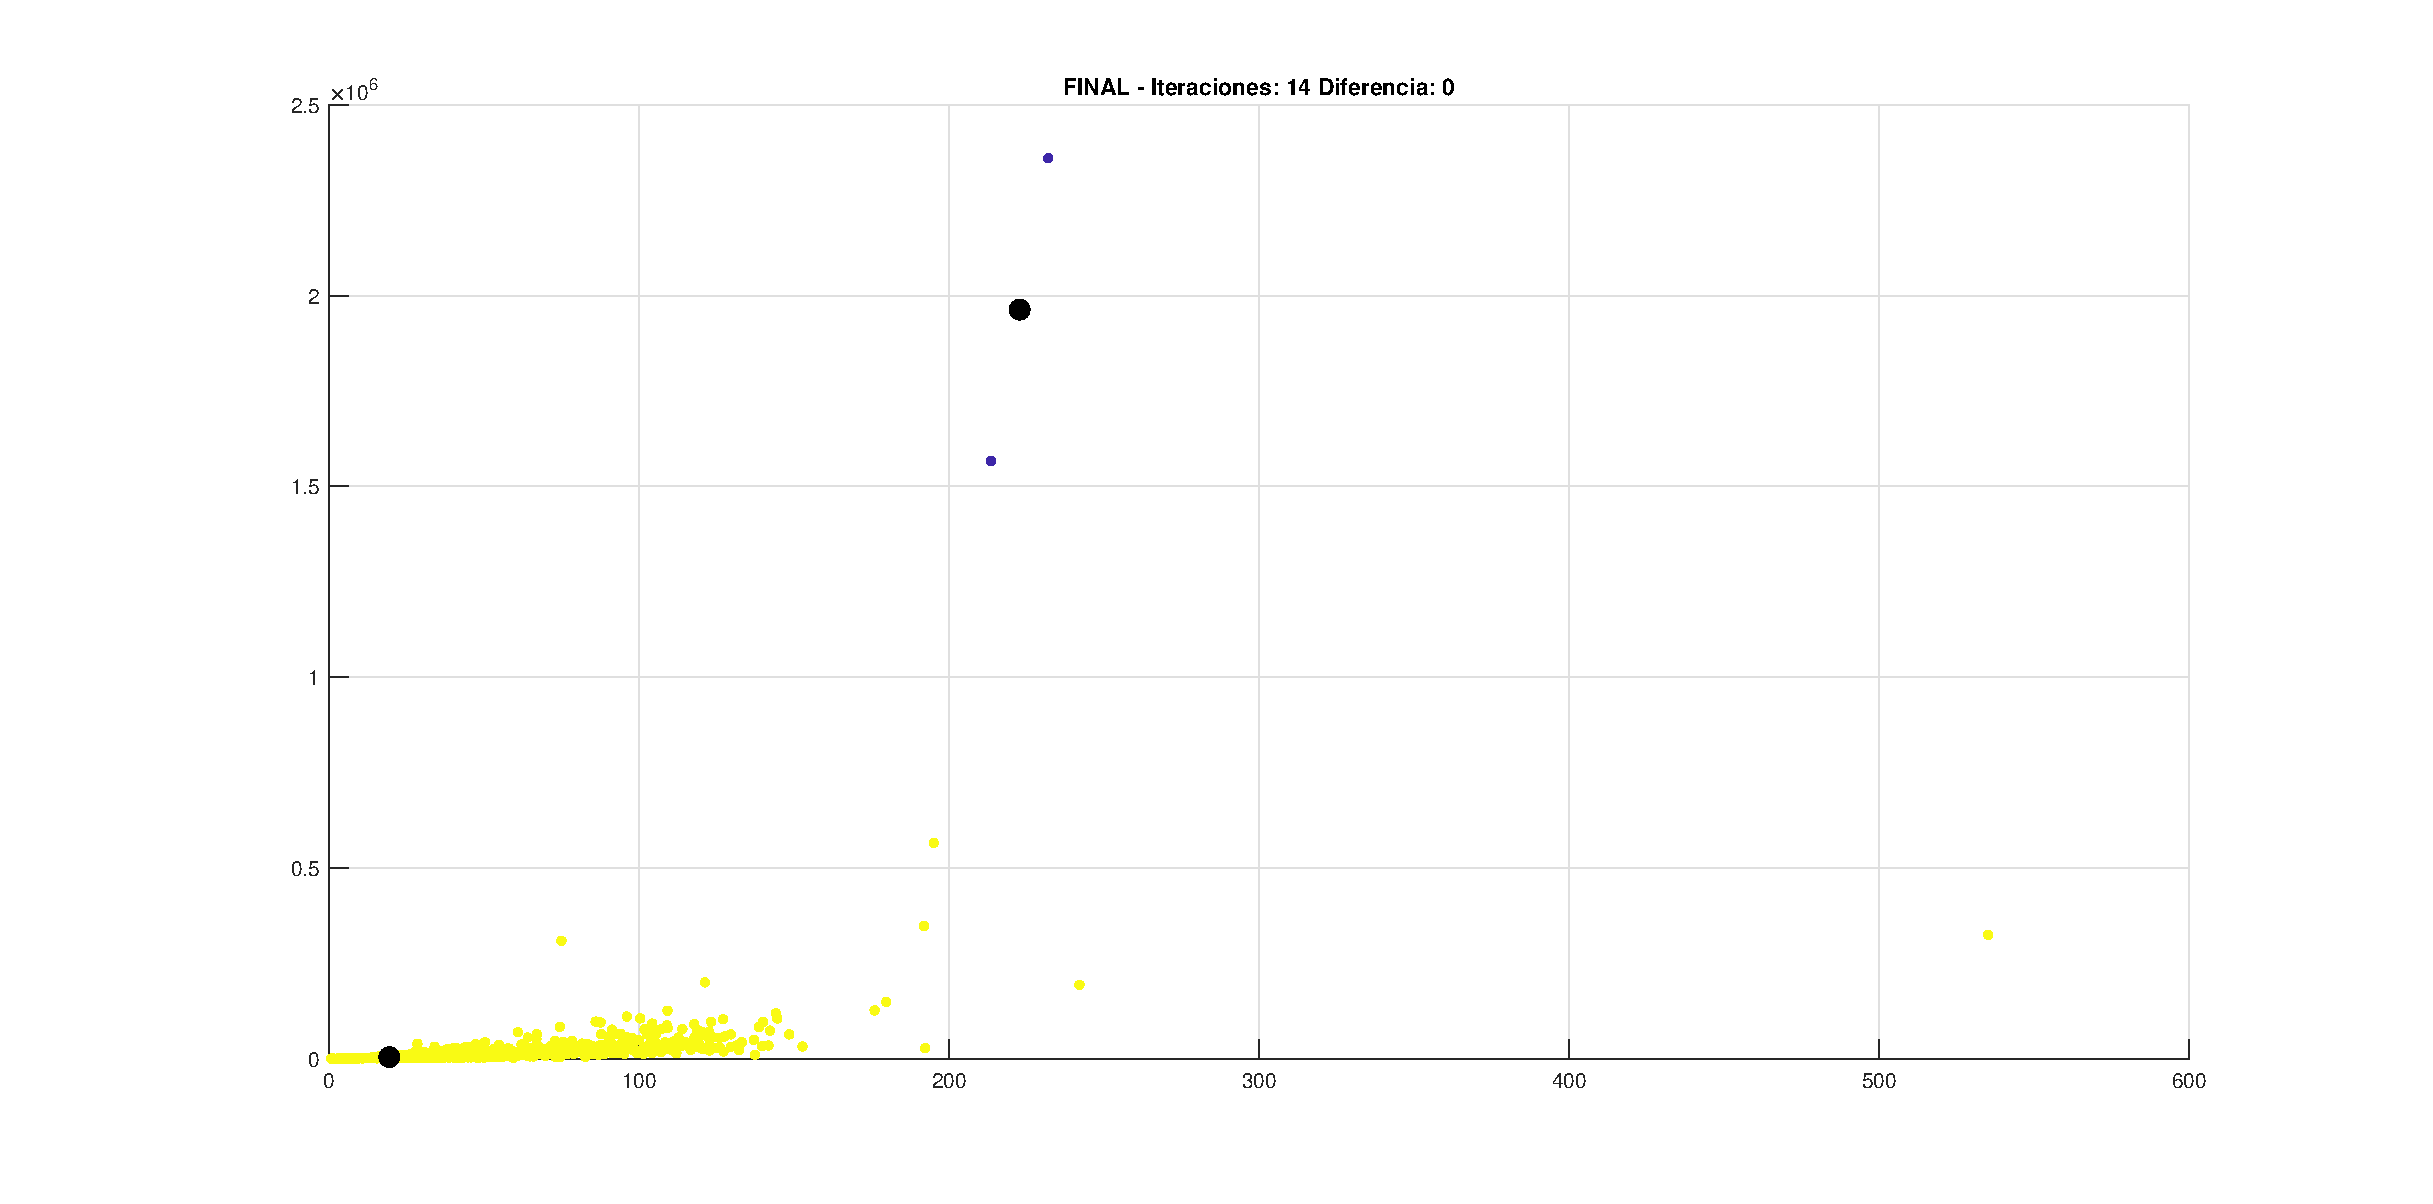
\includegraphics[width=0.90\textwidth]{figuras/k_means_time_4and5_sano_ictal.eps}
    \caption{Gráfica de agrupamiento por k-means de señales bioeléctricas de las características 4 y 5 en el dominio del tiempo de actividad ictal y no ictal.}
    \label{fig: k_means_time_4_5}
\end{figure}

\subsection{Resultados jerárquico}
Se observó que al aplicar el algoritmo de agrupación jerárquica a las características extraídas en el dominio del tiempo, los datos resultantes mostraron una disposición continua. 

En las Figuras~\ref{fig: jerar_Time_1_2} - \ref{fig: jerar_Time_3_4}, sugiriendo un comportamiento lineal en la distribución de las señales bioeléctricas. En cuanto a la Figura~\ref{fig: jerar_Time_1_4}, se percibe que los datos son muy similares entre ellos. Por lo que diferenciar clases es complejo utilizando las características 1 y 4. Por ultimo, como se observa en las Figuras~\ref{fig: jerar_Time_1_5} - \ref{fig: jerar_Time_4_5}, la combinación de la característica 5 con cualquier otra es altamente discriminatoria entre clases, además de, tener la peculiaridad que los datos se superponen, para la clase ictal. 

\begin{figure}[H]
    \centering
    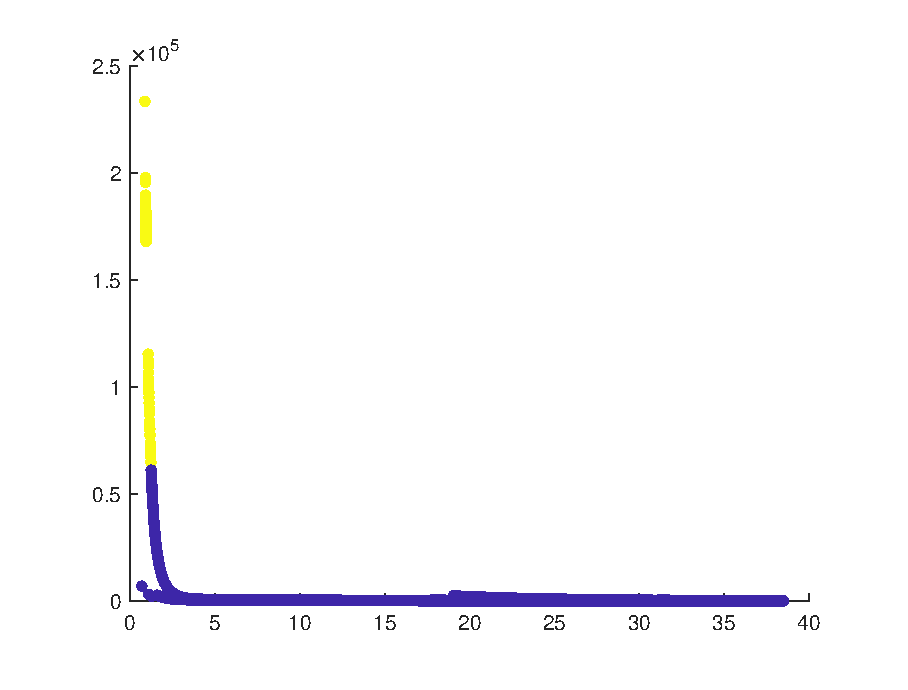
\includegraphics[width=0.7\textwidth]{figuras/jerar_time_1and_2_sano_ictal.eps}
    \caption{Gráfica de agrupamiento jerárquico de señales bioeléctricas de las características 1 y 2 en el dominio del tiempo  de actividad ictal y no ictal.}
    \label{fig: jerar_Time_1_2}
\end{figure}
\begin{figure}[H]
    \centering
    \includegraphics[width=0.7\textwidth]{figuras/jerar_time_1and_3_sano_ictal.eps}
    \caption{Gráfica de agrupamiento jerárquico de señales bioeléctricas de las características 1 y 3 en el dominio del tiempo  de actividad ictal y no ictal.}
    \label{fig: jerar_Time_1_3}
\end{figure}
\begin{figure}[H]
    \centering
    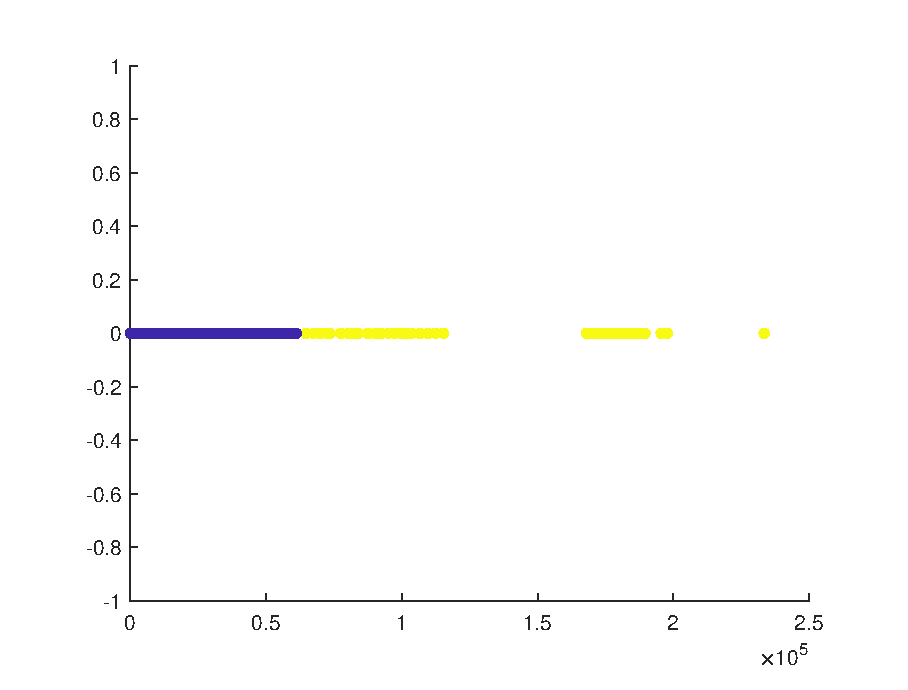
\includegraphics[width=0.7\textwidth]{figuras/jerar_time_2and_3_sano_ictal.eps}
    \caption{Gráfica de agrupamiento jerárquico de señales bioeléctricas de las características 2 y 3 en el dominio del tiempo  de actividad ictal y no ictal.}
    \label{fig: jerar_Time_2_3}
\end{figure}
\begin{figure}[H]
    \centering
    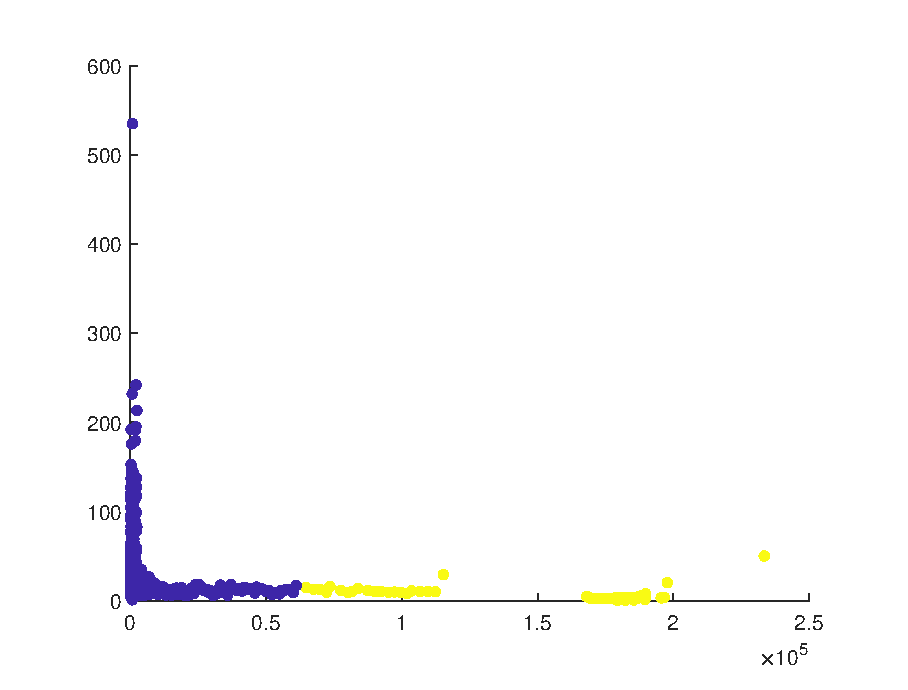
\includegraphics[width=0.7\textwidth]{figuras/jerar_time_2and_4_sano_ictal.eps}
    \caption{Gráfica de agrupamiento jerárquico de señales bioeléctricas de las características 2 y 4 en el dominio del tiempo  de actividad ictal y no ictal.}
    \label{fig: jerar_Time_2_4}
\end{figure}
\begin{figure}[H]
    \centering
    \includegraphics[width=0.7\textwidth]{figuras/jerar_time_3and_4_sano_ictal.eps}
    \caption{Gráfica de agrupamiento jerárquico de señales bioeléctricas de las características 3 y 4 en el dominio del tiempo  de actividad ictal y no ictal.}
    \label{fig: jerar_Time_3_4}
\end{figure}


\begin{figure}[H]
    \centering
    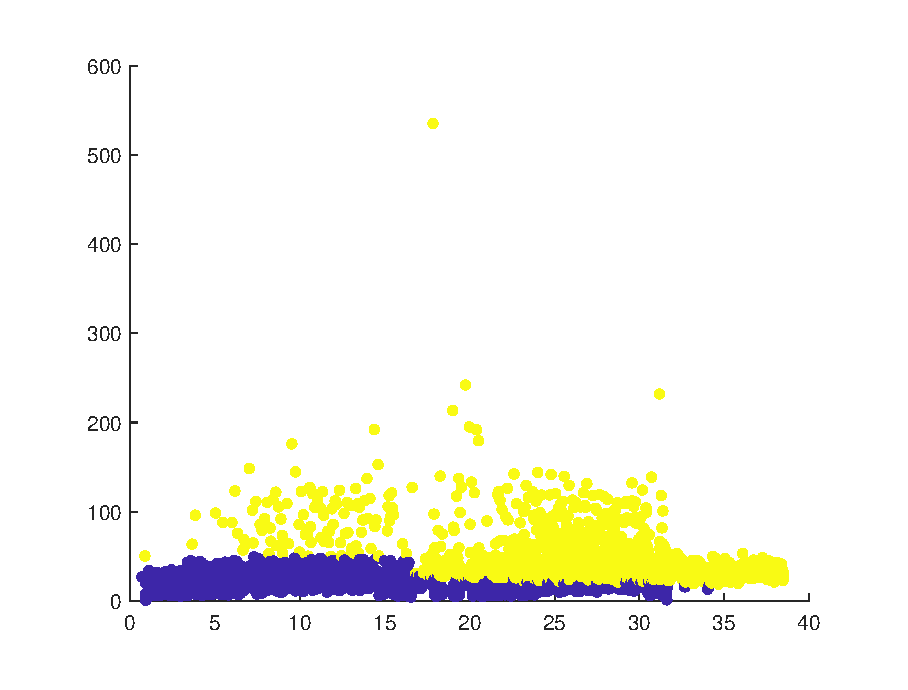
\includegraphics[width=0.7\textwidth]{figuras/jerar_time_1and_4_sano_ictal.eps}
    \caption{Gráfica de agrupamiento jerárquico de señales bioeléctricas de las características 1 y 4 en el dominio del tiempo  de actividad ictal y no ictal.}
    \label{fig: jerar_Time_1_4}
\end{figure}
\begin{figure}[H]
    \centering
    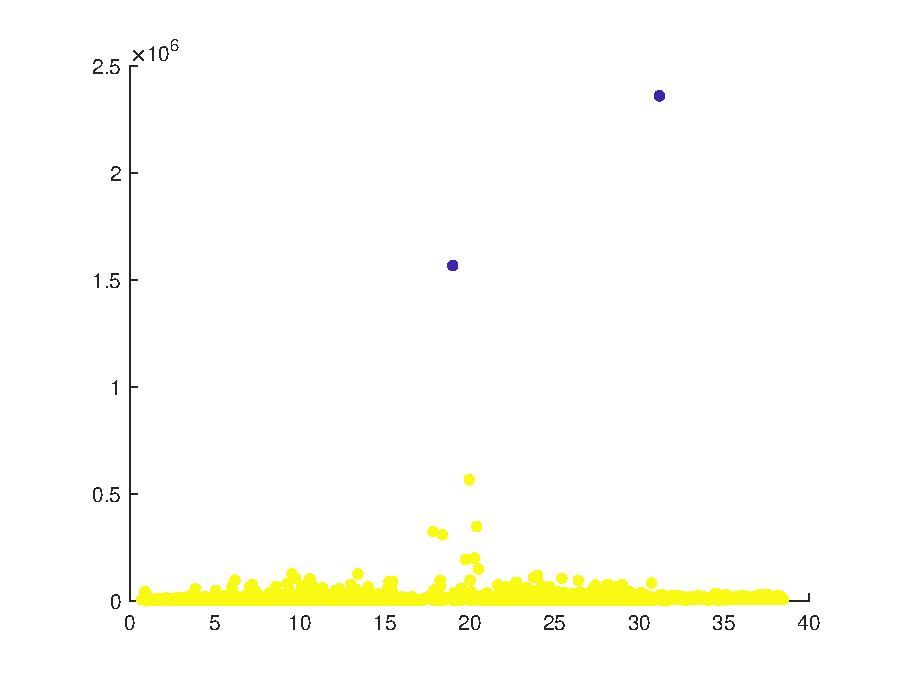
\includegraphics[width=0.7\textwidth]{figuras/jerar_time_1and_5_sano_ictal.eps}
    \caption{Gráfica de agrupamiento jerárquico de señales bioeléctricas de las características 1 y 5 en el dominio del tiempo  de actividad ictal y no ictal.}
    \label{fig: jerar_Time_1_5}
\end{figure}



\begin{figure}[H]
    \centering
    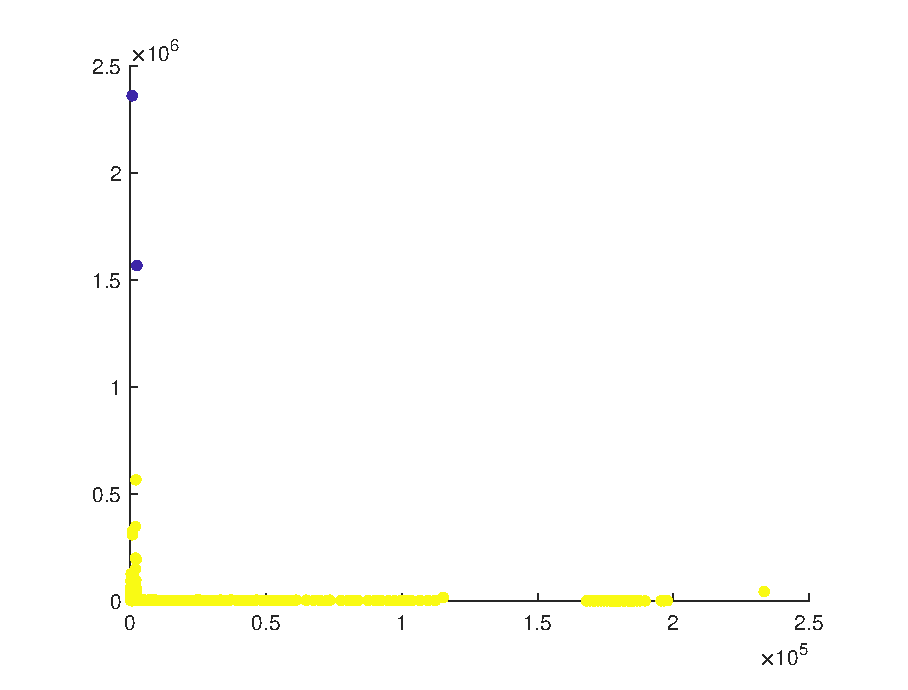
\includegraphics[width=0.7\textwidth]{figuras/jerar_time_2and_5_sano_ictal.eps}
    \caption{Gráfica de agrupamiento jerárquico de señales bioeléctricas de las características 2 y 5 en el dominio del tiempo  de actividad ictal y no ictal.}
    \label{fig: jerar_Time_2_5}
\end{figure}

\begin{figure}[H]
    \centering
    \includegraphics[width=0.7\textwidth]{figuras/jerar_time_3and_5_sano_ictal.eps}
    \caption{Gráfica de agrupamiento jerárquico de señales bioeléctricas de las características 3 y 5 en el dominio del tiempo  de actividad ictal y no ictal.}
    \label{fig: jerar_Time_3_5}
\end{figure}
\begin{figure}[H]
    \centering
    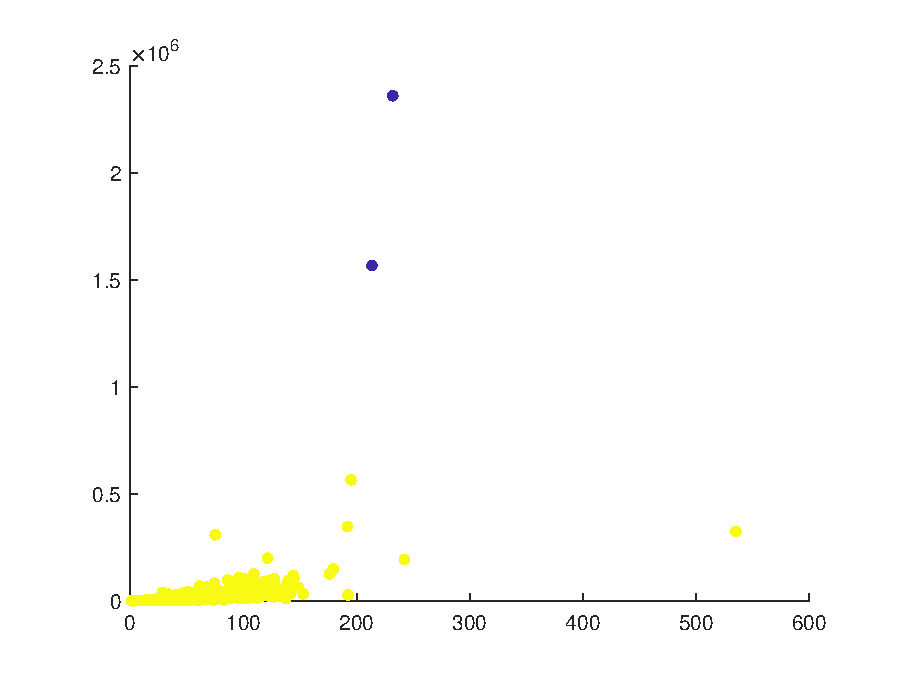
\includegraphics[width=0.7\textwidth]{figuras/jerar_time_4and_5_sano_ictal.eps}
    \caption{Gráfica de agrupamiento jerárquico de señales bioeléctricas de las características 4 y 5 en el dominio del tiempo  de actividad ictal y no ictal.}
    \label{fig: jerar_Time_4_5}
\end{figure}






\section{Análisis de Grupos en el Dominio de Frecuencia}
En el análisis de agrupamiento de señales EEG en el dominio de la frecuencia se trabajaron con las siguientes características:

\begin{enumerate}
    \item $\frac{\theta}{\alpha}$
    \item $\frac{\beta}{\alpha}$
    \item $\frac{\theta}{\beta}$
    \item $\frac{(\theta + \alpha)}{\beta}$
    \item $\frac{(\theta + \alpha)}{(\alpha + \beta)}$
    \item Desviación estándar
\end{enumerate}

%, \ref{fig: k_means_freq_1_3}, \ref{fig: k_means_freq_1_4}, \ref{fig: k_means_freq_1_5}, \ref{fig: k_means_freq_1_6}, \ref{fig: k_means_freq_2_3}, \ref{fig: k_means_freq_2_4}, \ref{fig: k_means_freq_2_5}, \ref{fig: k_means_freq_2_6}, \ref{fig: k_means_freq_3_4}, \ref{fig: k_means_freq_3_5}, \ref{fig: k_means_freq_3_6}, \ref{fig: k_means_freq_4_5},\ref{fig: k_means_freq_4_6} y

\subsection{Resultados K-means}
Los resultados fueron satisfactorios, como se puede observar en las Figuras~\ref{fig: k_means_freq_1_2} -  \ref{fig: k_means_freq_5_6}. Los datos forman un contorno similar a una elipse estirada por uno o dos bordes. Este patrón de agrupación resultó en una correcta separación de los datos en dos grupos, que consisten en señales EEG de individuos con actividad epiléptica y personas sanas. 

La capacidad de K-means para realizar esta separación respalda la validez de los resultados y sugiere la utilidad de las características de frecuencia en la discriminación entre individuos con actividad epiléptica y personas sanas, además de, poder notar que para este dominio la densidad de datos es muy similar para cada grupo. Por lo que el tener una mayor cantidad de datos y de manera diversificada (distintos pacientes) sin duda alguna se obtendrá una predicción excelente. 

Para las figuras anteriormente mencionadas en esta sección, cabe mencionar que con la transición entre cada grupo, se aprecia una disminución en la densidad de datos de manera gradual y significativa. Lo cual es esperado, ya que las grabaciones por parte de HUMANA contienen segmentos donde el paciente no esta pasando por un episodio epiléptico, lo que se interpretar como ruido en las características de su clase (ictal).

\begin{figure}[H]
    \centering
    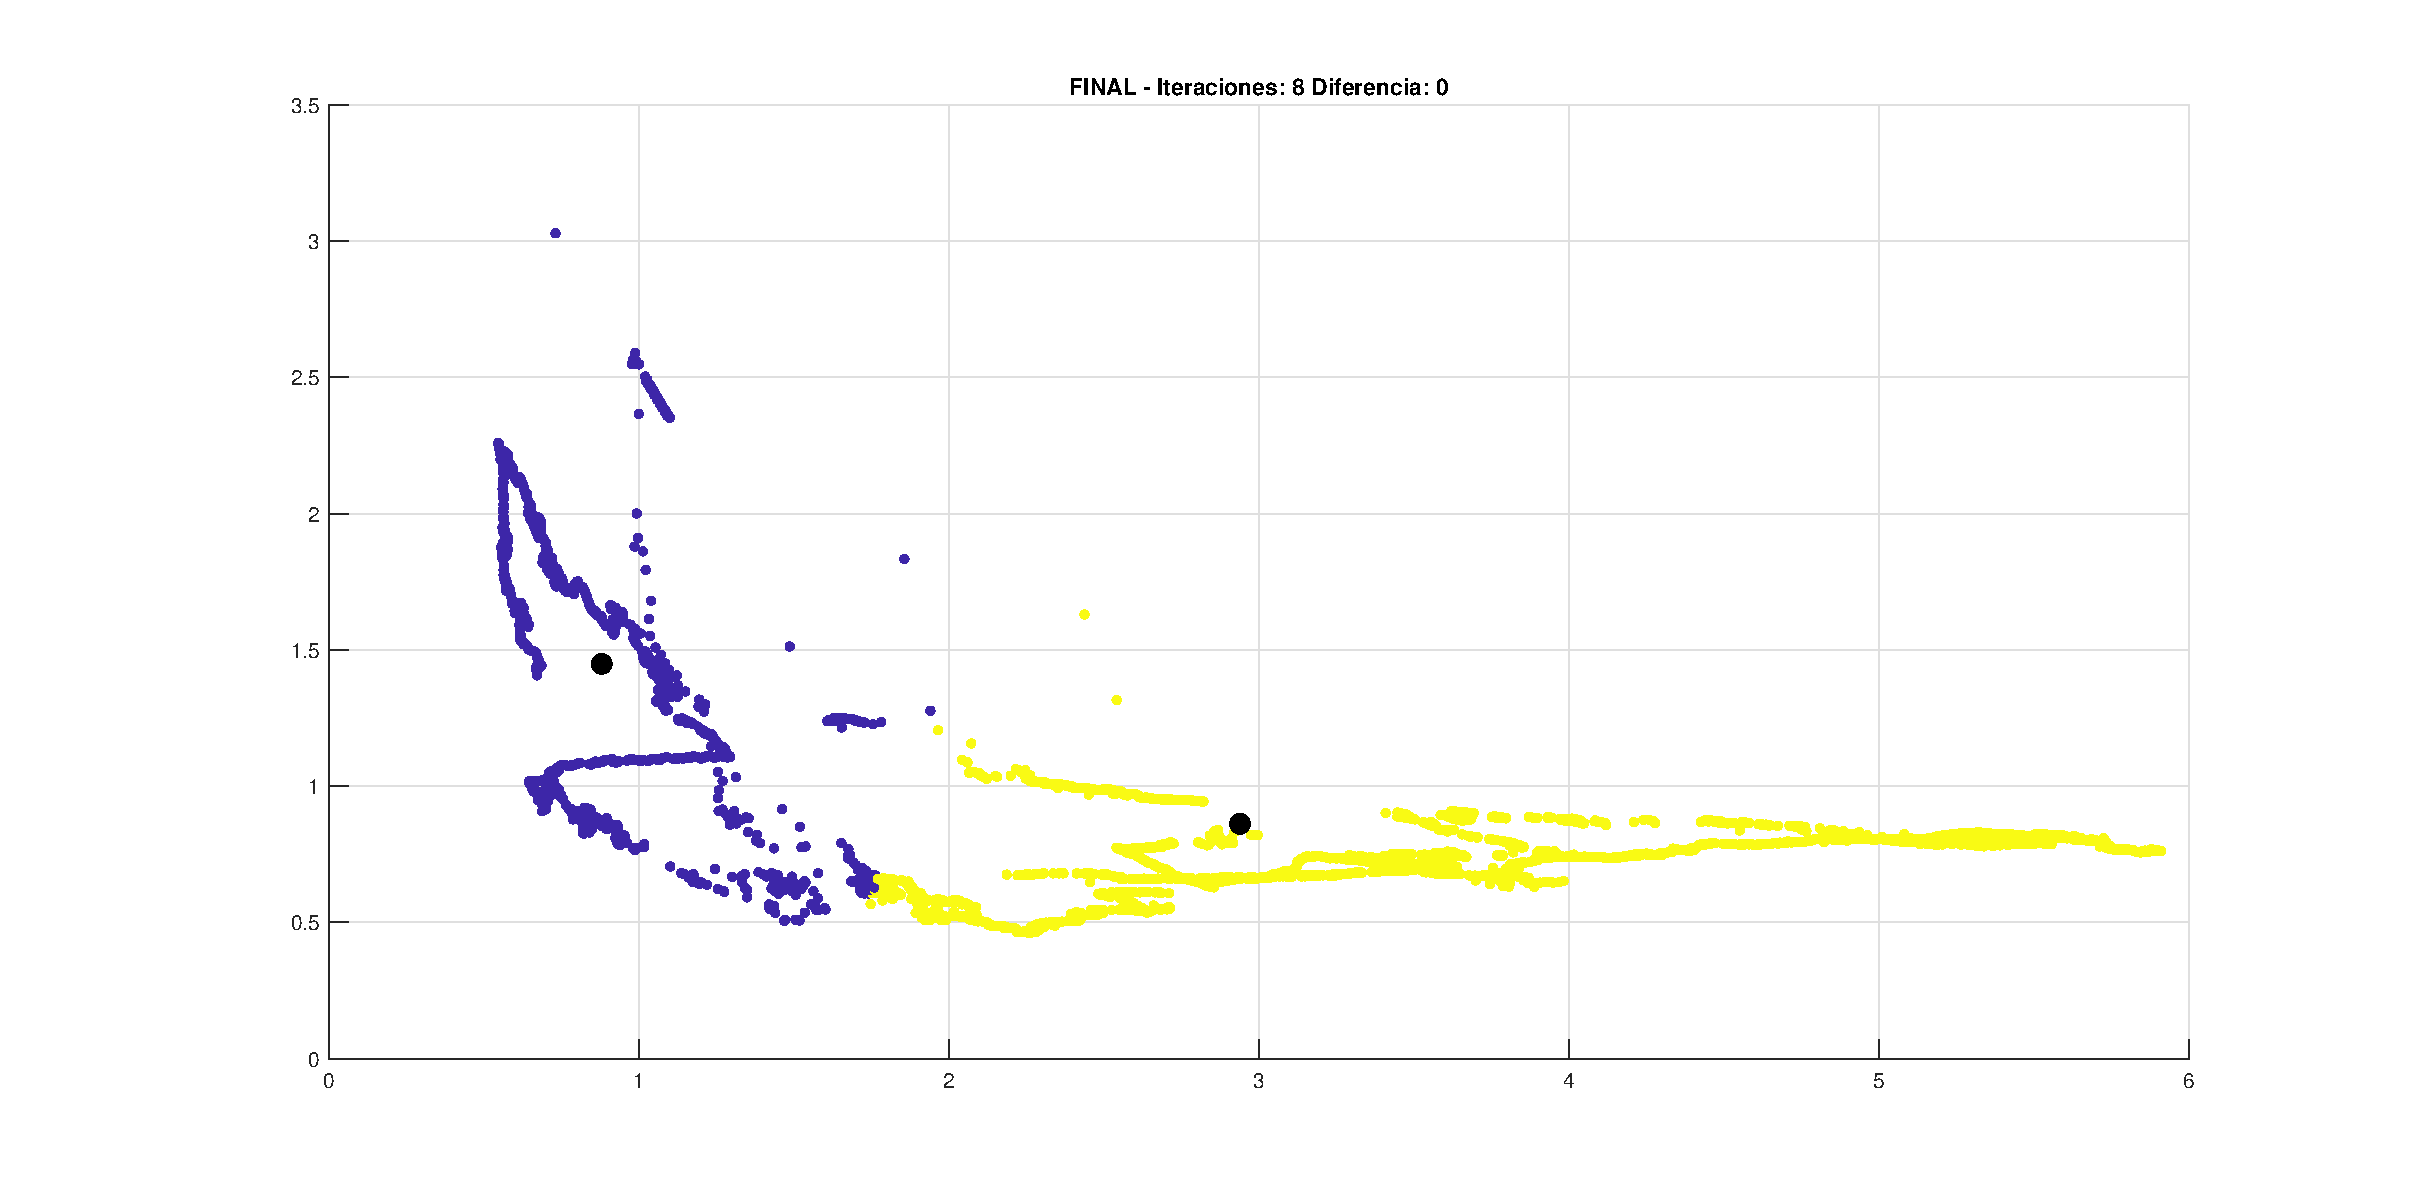
\includegraphics[width=0.90\textwidth]{figuras/k_means_freq_1and2_sano_ictal.eps}
    \caption{Gráfica de agrupamiento por k-means de señales bioeléctricas de las características 1 y 2 en el dominio de la frecuencia de actividad ictal y no ictal.}
    \label{fig: k_means_freq_1_2}
\end{figure}
\begin{figure}[H]
    \centering
    \includegraphics[width=0.80\textwidth]{figuras/k_means_freq_1and3_sano_ictal.eps}
    \caption{Gráfica de agrupamiento por k-means de señales bioeléctricas de las características 1 y 3 en el dominio de la frecuencia de actividad ictal y no ictal.}
    \label{fig: k_means_freq_1_3}
\end{figure}
\begin{figure}[H]
    \centering
    \includegraphics[width=0.90\textwidth]{figuras/k_means_freq_1and4_sano_ictal.eps}
    \caption{Gráfica de agrupamiento por k-means de señales bioeléctricas de las características 1 y 4 en el dominio de la frecuencia de actividad ictal y no ictal.}
    \label{fig: k_means_freq_1_4}
\end{figure}
\begin{figure}[H]
    \centering
    \includegraphics[width=0.8\textwidth]{figuras/k_means_freq_1and5_sano_ictal.eps}
    \caption{Gráfica de agrupamiento por k-means de señales bioeléctricas de las características 1 y 5  en el dominio de la frecuencia de actividad ictal y no ictal.}
    \label{fig: k_means_freq_1_5}
\end{figure}
\begin{figure}[H]
    \centering
    \includegraphics[width=0.8\textwidth]{figuras/k_means_freq_1and6_sano_ictal.eps}
    \caption{Gráfica de agrupamiento por k-means de señales bioeléctricas de las características 1 y 6 en el dominio de la frecuencia de actividad ictal y no ictal.}
    \label{fig: k_means_freq_1_6}
\end{figure}
\begin{figure}[H]
    \centering
    \includegraphics[width=0.8\textwidth]{figuras/k_means_freq_2and3_sano_ictal.eps}
    \caption{Gráfica de agrupamiento por k-means de señales bioeléctricas de las características 2 y 3 en el dominio de la frecuencia de actividad ictal y no ictal.}
    \label{fig: k_means_freq_2_3}
\end{figure}
\begin{figure}[H]
    \centering
    \includegraphics[width=0.8\textwidth]{figuras/k_means_freq_2and4_sano_ictal.eps}
    \caption{Gráfica de agrupamiento por k-means de señales bioeléctricas de las características 2 y 4 en el dominio de la frecuencia de actividad ictal y no ictal.}
    \label{fig: k_means_freq_2_4}
\end{figure}
\begin{figure}[H]
    \centering
    \includegraphics[width=0.8\textwidth]{figuras/k_means_freq_2and5_sano_ictal.eps}
    \caption{Gráfica de agrupamiento por k-means de señales bioeléctricas de las características 2 y 5 en el dominio de la frecuencia de actividad ictal y no ictal.}
    \label{fig: k_means_freq_2_5}
\end{figure}
\begin{figure}[H]
    \centering
    \includegraphics[width=0.8\textwidth]{figuras/k_means_freq_2and6_sano_ictal.eps}
    \caption{Gráfica de agrupamiento por k-means de señales bioeléctricas de las características 2 y 6 en el dominio de la frecuencia de actividad ictal y no ictal.}
    \label{fig: k_means_freq_2_6}
\end{figure}
\begin{figure}[H]
    \centering
    \includegraphics[width=0.8\textwidth]{figuras/k_means_freq_3and4_sano_ictal.eps}
    \caption{Gráfica de agrupamiento por k-means de señales bioeléctricas de las características 3 y 4 en el dominio de la frecuencia de actividad ictal y no ictal.}
    \label{fig: k_means_freq_3_4}
\end{figure}
\begin{figure}[H]
    \centering
    \includegraphics[width=0.8\textwidth]{figuras/k_means_freq_3and5_sano_ictal.eps}
    \caption{Gráfica de agrupamiento por k-means de señales bioeléctricas de las características 3 y 5 en el dominio de la frecuencia de actividad ictal y no ictal.}
    \label{fig: k_means_freq_3_5}
\end{figure}
\begin{figure}[H]
    \centering
    \includegraphics[width=0.8\textwidth]{figuras/k_means_freq_3and6_sano_ictal.eps}
    \caption{Gráfica de agrupamiento por k-means de señales bioeléctricas de las características 3 y 6 en el dominio de la frecuencia de actividad ictal y no ictal.}
    \label{fig: k_means_freq_3_6}
\end{figure}
\begin{figure}[H]
    \centering
    \includegraphics[width=0.8\textwidth]{figuras/k_means_freq_4and5_sano_ictal.eps}
    \caption{Gráfica de agrupamiento por k-means de señales bioeléctricas de las características 4 y 5 en el dominio de la frecuencia de actividad ictal y no ictal.}
    \label{fig: k_means_freq_4_5}
\end{figure}
\begin{figure}[H]
    \centering
    \includegraphics[width=0.8\textwidth]{figuras/k_means_freq_4and6_sano_ictal.eps}
    \caption{Gráfica de agrupamiento por k-means de señales bioeléctricas de las características 4 y 6 en el dominio de la frecuencia de actividad ictal y no ictal.}
    \label{fig: k_means_freq_4_6}
\end{figure}
\begin{figure}[H]
    \centering
    \includegraphics[width=0.8\textwidth]{figuras/k_means_freq_5and6_sano_ictal.eps}
    \caption{Gráfica de agrupamiento por k-means de señales bioeléctricas de las características 5 y 6 en el dominio de la frecuencia de actividad ictal y no ictal.}
    \label{fig: k_means_freq_5_6}
\end{figure}

\subsection{Resultados jerárquico}
Los resultados para este algoritmo de agrupación fueron exitosos como se puede observar en las Figuras~\ref{fig: jerar_freq_1_2} - \ref{fig: jerar_freq_5_6}. Respecto al algoritmo \textit{K-means} se percibe ligeras diferencias, siendo una de estas que la cantidad de épocas percibidas como clase ictal, aumenta considerablemente. Esto sugiere que el análisis de agrupamiento jerárquico, la estructura de árbol permite identificar relaciones de subgrupo dentro de las clases principales, capturando así patrones más complejos y sutiles en los datos. Además, el agrupamiento jerárquico no asume la misma forma esférica de los \textit{clusters} que hace \textit{k-means}, lo que le confiere una mayor flexibilidad para adaptarse a distribuciones de datos más complejas.

\begin{figure}[H]
    \centering
    \includegraphics[width=0.7\textwidth]{figuras/jerar_freq_1and_2_sano_ictal.eps}
    \caption{Gráfica de agrupamiento jerárquico de señales bioeléctricas de las características 1 y 2 en el dominio de la frecuencia de actividad ictal y no ictal.}
    \label{fig: jerar_freq_1_2}
\end{figure}
\begin{figure}[H]
    \centering
    \includegraphics[width=0.7\textwidth]{figuras/jerar_freq_1and_3_sano_ictal.eps}
    \caption{Gráfica de agrupamiento jerárquico de señales bioeléctricas de las características 1 y 3 en el dominio de la frecuencia de actividad ictal y no ictal.}
    \label{fig: jerar_freq_1_3}
\end{figure}

\begin{figure}[H]
    \centering
    \includegraphics[width=0.7\textwidth]{figuras/jerar_freq_1and_4_sano_ictal.eps}
    \caption{Gráfica de agrupamiento jerárquico de señales bioeléctricas de las características 1 y 4 en el dominio de la frecuencia de actividad ictal y no ictal.}
    \label{fig: jerar_freq_1_4}
\end{figure}
\begin{figure}[H]
    \centering
    \includegraphics[width=0.7\textwidth]{figuras/jerar_freq_1and_5_sano_ictal.eps}
    \caption{Gráfica de agrupamiento jerárquico de señales bioeléctricas de las características 1 y 5 en el dominio de la frecuencia de actividad ictal y no ictal.}
    \label{fig: jerar_freq_1_5}
\end{figure}
\begin{figure}[H]
    \centering
    \includegraphics[width=0.7\textwidth]{figuras/jerar_freq_1and_6_sano_ictal.eps}
    \caption{Gráfica de agrupamiento jerárquico de señales bioeléctricas de las características 1 y 6 en el dominio de la frecuencia de actividad ictal y no ictal.}
    \label{fig: jerar_freq_1_6}
\end{figure}
\begin{figure}[H]
    \centering
    \includegraphics[width=0.7\textwidth]{figuras/jerar_freq_2and_3_sano_ictal.eps}
    \caption{Gráfica de agrupamiento jerárquico de señales bioeléctricas de las características 2 y 3 en el dominio de la frecuencia de actividad ictal y no ictal.}
    \label{fig: jerar_freq_2_3}
\end{figure}
\begin{figure}[H]
    \centering
    \includegraphics[width=0.7\textwidth]{figuras/jerar_freq_2and_4_sano_ictal.eps}
    \caption{Gráfica de agrupamiento jerárquico de señales bioeléctricas de las características 2 y 4 en el dominio de la frecuencia de actividad ictal y no ictal.}
    \label{fig: jerar_freq_2_4}
\end{figure}
\begin{figure}[H]
    \centering
    \includegraphics[width=0.7\textwidth]{figuras/jerar_freq_2and_5_sano_ictal.eps}
    \caption{Gráfica de agrupamiento jerárquico de señales bioeléctricas de las características 2 y 5 en el dominio de la frecuencia de actividad ictal y no ictal.}
    \label{fig: jerar_freq_2_5}
\end{figure}
\begin{figure}[H]
    \centering
    \includegraphics[width=0.7\textwidth]{figuras/jerar_freq_2and_6_sano_ictal.eps}
    \caption{Gráfica de agrupamiento jerárquico de señales bioeléctricas de las características 2 y 6 en el dominio de la frecuencia de actividad ictal y no ictal.}
    \label{fig: jerar_freq_2_6}
\end{figure}
\begin{figure}[H]
    \centering
    \includegraphics[width=0.7\textwidth]{figuras/jerar_freq_3and_4_sano_ictal.eps}
    \caption{Gráfica de agrupamiento jerárquico de señales bioeléctricas de las características 3 y 4 en el dominio de la frecuencia de actividad ictal y no ictal.}
    \label{fig: jerar_freq_3_4}
\end{figure}
\begin{figure}[H]
    \centering
    \includegraphics[width=0.7\textwidth]{figuras/jerar_freq_3and_5_sano_ictal.eps}
    \caption{Gráfica de agrupamiento jerárquico de señales bioeléctricas de las características 3 y 5 en el dominio de la frecuencia de actividad ictal y no ictal.}
    \label{fig: jerar_freq_3_5}
\end{figure}
\begin{figure}[H]
    \centering
    \includegraphics[width=0.7\textwidth]{figuras/jerar_freq_3and_6_sano_ictal.eps}
    \caption{Gráfica de agrupamiento jerárquico de señales bioeléctricas de las características 3 y 6 en el dominio de la frecuencia de actividad ictal y no ictal.}
    \label{fig: jerar_freq_3_6}
\end{figure}
\begin{figure}[H]
    \centering
    \includegraphics[width=0.7\textwidth]{figuras/jerar_freq_4and_5_sano_ictal.eps}
    \caption{Gráfica de agrupamiento jerárquico de señales bioeléctricas de las características 4 y 5 en el dominio de la frecuencia de actividad ictal y no ictal.}
    \label{fig: jerar_freq_4_5}
\end{figure}
\begin{figure}[H]
    \centering
    \includegraphics[width=0.7\textwidth]{figuras/jerar_freq_4and_6_sano_ictal.eps}
    \caption{Gráfica de agrupamiento jerárquico de señales bioeléctricas de las características 4 y 6 en el dominio de la frecuencia de actividad ictal y no ictal.}
    \label{fig: jerar_freq_4_6}
\end{figure}
\begin{figure}[H]
    \centering
    \includegraphics[width=0.7\textwidth]{figuras/jerar_freq_5and_6_sano_ictal.eps}
    \caption{Gráfica de agrupamiento jerárquico de señales bioeléctricas de las características 5 y 6 en el dominio de la frecuencia de actividad ictal y no ictal.}
    \label{fig: jerar_freq_5_6}
\end{figure}


\section{Análisis de Grupos en el Dominio de Wavelets}
En esta sección, se aborda el análisis de grupos resultantes de la aplicación de técnicas de procesamiento en el dominio de wavelets. Se destacan las siguientes características utilizadas en el análisis:

\begin{enumerate}
    \item Potencia
    \item Desviación
    \item Asimetría
    \item Media
    \item Curtosis
    \item Cruces por cero (ZC)
\end{enumerate}

%, \ref{fig: k_means_wave_1_3}, \ref{fig: k_means_wave_1_4}, \ref{fig: k_means_wave_1_5}, \ref{fig: k_means_wave_1_6},

\subsection{Resultados K-means}
 La identificación de dos grupos de señales bioeléctricas que están ampliamente separados en el espacio de características es un hallazgo de gran relevancia, como se observa en las Figuras~\ref{fig: k_means_wave_1_2} - \ref{fig: k_means_wave_2_4}, \ref{fig: k_means_wave_2_6}, \ref{fig: k_means_wave_3_4}, \ref{fig: k_means_wave_3_6} - \ref{fig: k_means_wave_5_6}. Esta distinción evidente indica que las características analizadas, como la potencia, desviación, asimetría, media, curtosis y cruces por cero (ZC), son altamente discriminatorias entre las clases ictal y sana. Esta observación respalda la utilidad de estas características en la detección y diferenciación de estados epilépticos y salud.

La agrupación de datos en dos grupos cercanos, pero con diferentes características de densidad, también presenta un aspecto interesante, como se observar en las Figuras~\ref{fig: k_means_wave_2_3}, \ref{fig: k_means_wave_2_5} y \ref{fig: k_means_wave_3_5}. La concentración de datos en una región más pequeña en un grupo y su expansión en el otro indican que, si bien estos grupos están próximos, aún mantienen diferencias notables. Esta observación puede ser esclarecedora para la comprensión de las variaciones sutiles en las señales bioeléctricas y cómo estas variaciones pueden influir en la clasificación.

\begin{figure}[H]
    \centering
    \includegraphics[width=0.90\textwidth]{figuras/k_means_wavelet_1and2_sano_ictal.eps}
    \caption{Gráfica de agrupamiento por k-means de señales bioeléctricas de las características 1 y 2 tipo wavelets de actividad ictal y no ictal.}
    \label{fig: k_means_wave_1_2}
\end{figure}
\begin{figure}[H]
    \centering
    \includegraphics[width=0.8\textwidth]{figuras/k_means_wavelet_1and3_sano_ictal.eps}
    \caption{Gráfica de agrupamiento por k-means de señales bioeléctricas de las características 1 y 3 tipo wavelets de actividad ictal y no ictal.}
    \label{fig: k_means_wave_1_3}
\end{figure}
\begin{figure}[H]
    \centering
    \includegraphics[width=0.8\textwidth]{figuras/k_means_wavelet_1and4_sano_ictal.eps}
    \caption{Gráfica de agrupamiento por k-means de señales bioeléctricas de las características 1 y 4  tipo wavelets de actividad ictal y no ictal.}
    \label{fig: k_means_wave_1_4}
\end{figure}
\begin{figure}[H]
    \centering
    \includegraphics[width=0.8\textwidth]{figuras/k_means_wavelet_1and5_sano_ictal.eps}
    \caption{Gráfica de agrupamiento por k-means de señales bioeléctricas de las características 1 y 5 tipo wavelets de actividad ictal y no ictal.}
    \label{fig: k_means_wave_1_5}
\end{figure}
\begin{figure}[H]
    \centering
    \includegraphics[width=0.8\textwidth]{figuras/k_means_wavelet_1and6_sano_ictal.eps}
    \caption{Gráfica de agrupamiento por k-means de señales bioeléctricas de las características 1 y 6 tipo wavelets de actividad ictal y no ictal.}
    \label{fig: k_means_wave_1_6}
\end{figure}
\begin{figure}[H]
    \centering
    \includegraphics[width=0.8\textwidth]{figuras/k_means_wavelet_2and3_sano_ictal.eps}
    \caption{Gráfica de agrupamiento por k-means de señales bioeléctricas de las características 2 y 3 tipo wavelets de actividad ictal y no ictal.}
    \label{fig: k_means_wave_2_3}
\end{figure}
\begin{figure}[H]
    \centering
    \includegraphics[width=0.8\textwidth]{figuras/k_means_wavelet_2and4_sano_ictal.eps}
    \caption{Gráfica de agrupamiento por k-means de señales bioeléctricas de las características 2 y 4 tipo wavelets de actividad ictal y no ictal.}
    \label{fig: k_means_wave_2_4}
\end{figure}
\begin{figure}[H]
    \centering
    \includegraphics[width=0.8\textwidth]{figuras/k_means_wavelet_2and5_sano_ictal.eps}
    \caption{Gráfica de agrupamiento por k-means de señales bioeléctricas de las características 2 y 5 tipo wavelets de actividad ictal y no ictal.}
    \label{fig: k_means_wave_2_5}
\end{figure}
\begin{figure}[H]
    \centering
    \includegraphics[width=0.8\textwidth]{figuras/k_means_wavelet_2and6_sano_ictal.eps}
    \caption{Gráfica de agrupamiento por k-means de señales bioeléctricas de las características 2 y 6 tipo wavelets de actividad ictal y no ictal.}
    \label{fig: k_means_wave_2_6}
\end{figure}
\begin{figure}[H]
    \centering
    \includegraphics[width=0.8\textwidth]{figuras/k_means_wavelet_3and4_sano_ictal.eps}
    \caption{Gráfica de agrupamiento por k-means de señales bioeléctricas de las características 3 y 4 tipo wavelets de actividad ictal y no ictal.}
    \label{fig: k_means_wave_3_4}
\end{figure}
\begin{figure}[H]
    \centering
    \includegraphics[width=0.8\textwidth]{figuras/k_means_wavelet_3and5_sano_ictal.eps}
    \caption{Gráfica de agrupamiento por k-means de señales bioeléctricas de las características 3 y 5 tipo wavelets de actividad ictal y no ictal.}
    \label{fig: k_means_wave_3_5}
\end{figure}
\begin{figure}[H]
    \centering
    \includegraphics[width=0.8\textwidth]{figuras/k_means_wavelet_3and6_sano_ictal.eps}
    \caption{Gráfica de agrupamiento por k-means de señales bioeléctricas de las características 3 y 6 tipo wavelets de actividad ictal y no ictal.}
    \label{fig: k_means_wave_3_6}
\end{figure}
\begin{figure}[H]
    \centering
    \includegraphics[width=0.8\textwidth]{figuras/k_means_wavelet_4and5_sano_ictal.eps}
    \caption{Gráfica de agrupamiento por k-means de señales bioeléctricas de las características 4 y 5 tipo wavelets de actividad ictal y no ictal.}
    \label{fig: k_means_wave_4_5}
\end{figure}
\begin{figure}[H]
    \centering
    \includegraphics[width=0.8\textwidth]{figuras/k_means_wavelet_4and6_sano_ictal.eps}
    \caption{Gráfica de agrupamiento por k-means de señales bioeléctricas de las características 4 y 6 tipo wavelets de actividad ictal y no ictal.}
    \label{fig: k_means_wave_4_6}
\end{figure}
\begin{figure}[H]
    \centering
    \includegraphics[width=0.8\textwidth]{figuras/k_means_wavelet_5and6_sano_ictal.eps}
    \caption{Gráfica de agrupamiento por k-means de señales bioeléctricas de las características 5 y 6 tipo wavelets de actividad ictal y no ictal.}
    \label{fig: k_means_wave_5_6}
\end{figure}

\subsection{Resultados jerárquicos}
Como se puede observar en las Figuras~\ref{fig: jerar_freq_1_2} - \ref{fig: jerar_wave_5_6}, los resultados fueron exitosos, al ser altamente discriminatorios para cada tipo de clase. Se puede notar también que independientemente del algoritmo de agrupamiento empleado para realizar los modelos, se obtendrán resultados muy similares cuando se utilizan características wavelets. 

\begin{figure}[H]
    \centering
    \includegraphics[width=0.7\textwidth]{figuras/jerar_wavelets_1and_2_sano_ictal.eps}
    \caption{Gráfica de agrupamiento jerárquico de señales bioeléctricas de las características 1 y 2 tipo wavelets de actividad ictal y no ictal.}
    \label{fig: jerar_wave_1_2}
\end{figure}
\begin{figure}[H]
    \centering
    \includegraphics[width=0.7\textwidth]{figuras/jerar_wavelets_1and_3_sano_ictal.eps}
    \caption{Gráfica de agrupamiento jerárquico de señales bioeléctricas de las características 1 y 3 tipo wavelets de actividad ictal y no ictal.}
    \label{fig: jerar_wave_1_3}
\end{figure}
\begin{figure}[H]
    \centering
    \includegraphics[width=0.7\textwidth]{figuras/jerar_wavelets_1and_4_sano_ictal.eps}
    \caption{Gráfica de agrupamiento jerárquico de señales bioeléctricas de las características 1 y 4 tipo wavelets de actividad ictal y no ictal.}
    \label{fig: jerar_wave_1_4}
\end{figure}
\begin{figure}[H]
    \centering
    \includegraphics[width=0.7\textwidth]{figuras/jerar_wavelets_1and_5_sano_ictal.eps}
    \caption{Gráfica de agrupamiento jerárquico de señales bioeléctricas de las características 1 y 5 tipo wavelets de actividad ictal y no ictal.}
    \label{fig: jerar_wave_1_5}
\end{figure}
\begin{figure}[H]
    \centering
    \includegraphics[width=0.7\textwidth]{figuras/jerar_wavelets_1and_6_sano_ictal.eps}
    \caption{Gráfica de agrupamiento jerárquico de señales bioeléctricas de las características 1 y 6 tipo wavelets de actividad ictal y no ictal.}
    \label{fig: jerar_wave_1_6}
\end{figure}
\begin{figure}[H]
    \centering
    \includegraphics[width=0.7\textwidth]{figuras/jerar_wavelets_2and_3_sano_ictal.eps}
    \caption{Gráfica de agrupamiento jerárquico de señales bioeléctricas de las características 2 y 3 tipo wavelets de actividad ictal y no ictal.}
    \label{fig: jerar_wave_2_3}
\end{figure}
\begin{figure}[H]
    \centering
    \includegraphics[width=0.7\textwidth]{figuras/jerar_wavelets_2and_4_sano_ictal.eps}
    \caption{Gráfica de agrupamiento jerárquico de señales bioeléctricas de las características 2 y 4 tipo wavelets de actividad ictal y no ictal.}
    \label{fig: jerar_wave_2_4}
\end{figure}
\begin{figure}[H]
    \centering
    \includegraphics[width=0.7\textwidth]{figuras/jerar_wavelets_2and_5_sano_ictal.eps}
    \caption{Gráfica de agrupamiento jerárquico de señales bioeléctricas de las características 2 y 5 tipo wavelets de actividad ictal y no ictal.}
    \label{fig: jerar_wave_2_5}
\end{figure}

\begin{figure}[H]
    \centering
    \includegraphics[width=0.7\textwidth]{figuras/jerar_wavelets_2and_6_sano_ictal.eps}
    \caption{Gráfica de agrupamiento jerárquico de señales bioeléctricas de las características 2 y 6 tipo wavelets de actividad ictal y no ictal.}
    \label{fig: jerar_wave_2_6}
\end{figure}
\begin{figure}[H]
    \centering
    \includegraphics[width=0.7\textwidth]{figuras/jerar_wavelets_3and_4_sano_ictal.eps}
    \caption{Gráfica de agrupamiento jerárquico de señales bioeléctricas de las características 3 y 4 tipo wavelets de actividad ictal y no ictal.}
    \label{fig: jerar_wave_3_4}
\end{figure}
\begin{figure}[H]
    \centering
    \includegraphics[width=0.7\textwidth]{figuras/jerar_wavelets_3and_5_sano_ictal.eps}
    \caption{Gráfica de agrupamiento jerárquico de señales bioeléctricas de las características 3 y 5 tipo wavelets de actividad ictal y no ictal.}
    \label{fig: jerar_wave_3_5}
\end{figure}
\begin{figure}[H]
    \centering
    \includegraphics[width=0.7\textwidth]{figuras/jerar_wavelets_3and_6_sano_ictal.eps}
    \caption{Gráfica de agrupamiento jerárquico de señales bioeléctricas de las características 3 y 6 tipo wavelets de actividad ictal y no ictal.}
    \label{fig: jerar_wave_3_6}
\end{figure}
\begin{figure}[H]
    \centering
    \includegraphics[width=0.7\textwidth]{figuras/jerar_wavelets_4and_5_sano_ictal.eps}
    \caption{Gráfica de agrupamiento jerárquico de señales bioeléctricas de las características 4 y 5 tipo wavelets de actividad ictal y no ictal.}
    \label{fig: jerar_wave_4_5}
\end{figure}
\begin{figure}[H]
    \centering
    \includegraphics[width=0.7\textwidth]{figuras/jerar_wavelets_4and_6_sano_ictal.eps}
    \caption{Gráfica de agrupamiento jerárquico de señales bioeléctricas de las características 4 y 6 tipo wavelets de actividad ictal y no ictal.}
    \label{fig: jerar_wave_4_6}
\end{figure}
\begin{figure}[H]
    \centering
    \includegraphics[width=0.7\textwidth]{figuras/jerar_wavelets_5and_6_sano_ictal.eps}
    \caption{Gráfica de agrupamiento jerárquico de señales bioeléctricas de las características 5 y 6 tipo wavelets de actividad ictal y no ictal.}
    \label{fig: jerar_wave_5_6}
\end{figure}

\section{Herramienta para la evaluación visual de la tendencia}
Se añadió la herramienta ``VAT: \textit{ A Tool for Visual Assessment of (Cluster) Tendency}'' como una herramienta valiosa para la evaluación visual de la tendencia de agrupación de datos en señales bioeléctricas como se observa en la Figura~\ref{fig: Vat_toolbox}. Esta herramienta desempeñó un papel esencial al proporcionar una representación visual clara de la estructura de agrupación de datos en múltiples dimensiones. Su uso se justifica en la necesidad de comprender la tendencia de agrupación en un conjunto de características que puede ser complejo y visualmente abrumador al aplicar técnicas de agrupamiento como K-means o jerárquico.

\begin{figure}[H]
	\centering
	\includegraphics[width=0.6\textwidth]{figuras/39_VAT.png}
	\caption{VAT en la herramienta de software para el estudio de la epilepsia.}
	\label{fig: Vat_toolbox}
\end{figure}

Para la aplicación de VAT se utilizaron los vectores de características completos, mencionados en el capitulo anterior. 
Como se puede observar en la Figura~\ref{fig: Vat_time} no es posible determinar una cantidad de grupos para las características en el dominio del tiempo. Lo cual implica que todos los datos independientemente de su clase (ictal o sano) están muy cerca unos de otros. Permitiendo así validar de forma visual que las características en el dominio del tiempo de las señales EEG no son las más optimas. 

En el caso de las características en el dominio de la frecuencia, revelaron ser más discriminatorias como se puede observar en la Figura~\ref{fig: Vat_freq}. Se perciben varias subgrupos los cuales pertenecen a cada tipo de característica y clase. Se puede inferir que las características en el dominio de la frecuencia presentan un mejor comportamiento para realizar predicciones correctas. En cuanto a las características wavelets, son las que mejor discriminación realizan entre clases, como se puede observar en la Figura~\ref{fig: Vat_wavelet}. Dejando bastante evidente la cantidad de clases que existen en el vector de características.

En las Figuras~\ref{fig: Vat_freq} y \ref{fig: Vat_wavelet}, se puede percibir que a la fecha no se cuenta con la misma cantidad de grabaciones de personas Ictales respecto a grabaciones de personas sanas. 

La aplicación de ``VAT'' permitió una evaluación efectiva de la tendencia de agrupación en los datos de señales bioeléctricas. Los resultados generados por esta herramienta se alinearon con las expectativas teóricas y ayudaron a identificar patrones de agrupación en el conjunto de datos y visualizar el ruido que se puede encontrar entre los tipos de clases. Esta validación refuerza la fiabilidad y utilidad de la herramienta ``VAT'' en el contexto de este estudio y respalda su contribución a la comprensión de la tendencia de agrupación en señales bioeléctricas.  En los anexos se presentan resultados adicionales a los presentados en esta sección.


\begin{figure}[H]
	\centering
	\includegraphics[width=0.75\textwidth]{figuras/vat_edf_n_Uban15_time.eps}
	\caption{Resultado tras aplicar VAT al vector de características de 5 dimensiones en el dominio tiempo.}
	\label{fig: Vat_time}
\end{figure}
\begin{figure}[H]
	\centering
	\includegraphics[width=0.75\textwidth]{figuras/vat_edf_n_Uban15_freq.eps}
	\caption{Resultado tras aplicar VAT al vector de características de 6 dimensiones en el dominio frecuencia.}
	\label{fig: Vat_freq}
\end{figure}
\begin{figure}[H]
	\centering
	\includegraphics[width=0.8\textwidth]{figuras/vat_edf_n_Uban15_wavelet.eps}
	\caption{Resultado tras aplicar VAT al vector de características de 6 dimensiones en el dominio wavelets.}
	\label{fig: Vat_wavelet}
\end{figure}



\chapter{Actualización de la herramienta de software para el estudio de la epilepsia}
La actualización de la herramienta de software para el estudio de la epilepsia ha resultado en una herramienta más simple de actualizar, ya que los códigos están mejor comentados lo que ayuda definitivamente para la documentación y modificación del mismo. La herramienta ahora cuenta con más programación defensiva, lo cual es de gran ayuda a que la herramienta de software para el estudio de la epilepsia no colapse cuando se produce una advertencia o error inesperado, o por el mal uso de la misma herramienta.

Con las actualizaciones hechas, la herramienta tiene las siguientes características:
\begin{itemize}
    \item Un software más liviano: al no contar con funciones y variables innecesarias, además de, contar con métodos más sofisticados para realizar tareas en especifico y funciones nativas de MATLAB que se han descontinuado. 
    \item Facilidad para manipulación de datos: para la importación y exportación de datos, ya que en la actual versión se pueden importar datos del tipo ``edf'', ``MAT'' y de la base de datos local. La exportación de datos se da en formato ``MAT'', ``XLSX'' y ``CSV''.
\end{itemize}

Se implementó una funcionalidad crucial para mejorar la experiencia del usuario: la incorporación de ventanas de avisos. Estas notificaciones están diseñadas para mantener informado al usuario sobre las acciones en curso dentro de la herramienta de software, como se observa en la Figura~\ref{fig: avisos_toolbox}. Además, ofrecen indicaciones sobre el progreso de procesos extensos, alertan sobre la necesidad de esperar durante operaciones específicas y notifican cualquier problema o inconveniente que pueda surgir durante el uso de la herramienta. Esta adición no solo busca proporcionar una interacción más transparente, sino también brindar al usuario un mayor control y comprensión de las operaciones realizadas en la herramienta de software.

\begin{figure}[H]
    \centering
    \includegraphics[width=0.4\textwidth]{figuras/44_ventana_aviso.png}
    \caption{Ventana de avisos.}
    \label{fig: avisos_toolbox}
\end{figure}

En el marco del continuo desarrollo y mejora de la herramienta de software, se ha integrado una funcionalidad fundamental para facilitar la comprensión y el depurado del sistema. Ahora, la consola de MATLAB presenta mensajes y anuncios, proporcionando información sobre las acciones que se están llevando a cabo dentro de la herramienta de software. Esta característica no solo contribuye al desarrollo continuo del software, sino que también facilita el proceso de depuración, permitiendo a los desarrolladores identificar y abordar eficientemente cualquier problema que pueda surgir durante la ejecución. Dicha inclusión de mensajes en la consola respalda así un entorno de desarrollo más efectivo y eficiente, observese la Figura~\ref{fig: debbug_matlab}.

\begin{figure}[H]
    \centering
    \includegraphics[width=0.65\textwidth]{figuras/46_notes_debug.png}
    \caption{Notas en consola de MATLAB.}
    \label{fig: debbug_matlab}
\end{figure}

La presente versión de la herramienta de software para el estudio de la epilepsia concluirá siendo implementada en el trabajo de graduación de Diego Méndez titulado ``Extensión, validación y migración de una herramienta de software para el estudio de la epilepsia para su uso en el Centro de Epilepsia y Neurocirugía Funcional HUMANA)''~\cite{diego_2023}. Dicha implementación permitirá obtener una herramienta de software para el estudio de la epilepsia capaz de ser ejecutada en cualquier computadora siendo amigable con el usuario, además de contar con una base de datos local.  


